%Version 3.1 December 2024
\RequirePackage{silence}
\WarningFilter{hyperref}{Difference}
\documentclass[pdflatex,sn-mathphys-num]{sn-jnl}% Math and Physical Sciences Numbered Reference Style
\usepackage{graphicx}%
\usepackage{multirow}%
\usepackage{amsmath,amssymb,amsfonts}%
\usepackage{amsthm}%

\usepackage[title]{appendix}%
\usepackage{xcolor}%
\usepackage{textcomp}%
\usepackage{manyfoot}%
\usepackage{booktabs}%
\usepackage{algorithm}%
\usepackage{algorithmicx}%
\usepackage{algpseudocode}%
\usepackage{listings}%
\usepackage{tabularx} % Add to preamble
\usepackage{microtype}
\emergencystretch=3em
\theoremstyle{thmstyleone}%
\newtheorem{theorem}{Theorem}%
\newtheorem{proposition}[theorem]{Proposition}%
\newtheorem{assumption}{Assumption}%

\theoremstyle{thmstyletwo}%
\newtheorem{example}{Example}%
\newtheorem{remark}{Remark}%

\theoremstyle{thmstylethree}%
\newtheorem{definition}{Definition}%

\raggedbottom
\makeatletter
\def\toclevel@paragraph{3} % prevents level-skip warnings from \subsection -> \paragraph
\makeatother
\begin{document}
\sloppy

\title[Spectral Flattening as a Security Guarantee: Hyperchaotic Speech Encryption with Constrained Genetic Keystream Certification for IoT Audio Devices]{Spectral Flattening as a Security Guarantee: Hyperchaotic Speech Encryption with Constrained Genetic Keystream Certification for IoT Audio Devices}

\author[1]{\fnm{Harshit} \sur{S Jain}}\email{harshitj3235@gmail.com}

\author[1]{\fnm{Aayushi R} \sur{}}\email{aayushirrjain@gmail.com}

\author[1]{\fnm{Yash Jain} \sur{}}\email{yashjain5108@gmail.com}

\author*[2]{\fnm{Ambili} \sur{K N}}\email{ambilikn@gmail.com}

\author*[3]{\fnm{Praveen} \sur{K}}\email{k\_praveen@cb.amrita.edu}

\author[1]{\fnm{Anirudha} \sur{Prabhu}}\email{aniprabhubp@gmail.com}


\affil[1]{\orgdiv{Department of Computer Science and Engineering}, \orgname{Jain University}, \orgaddress{\street{Kanakapura Road}, \city{Ramanagara District}, \postcode{562112}, \state{Karnataka}, \country{India}}}

\affil*[2]{\orgdiv{Department of CSE-Cyber Security}, \orgname{Dayananda Sagar Academy of Technology and Management}, \orgaddress{ \city{Bengaluru}, \postcode{560082}, \state{Karnataka}, \country{India}}}

\affil*[3]{\orgdiv{TIFAC CORE in Cyber Security}, \orgname{Amrita Vishwa Vidyapeetham}, \orgaddress{ \city{Coimbatore},\state{Tamil Nadu}, \country{India}}}

\abstract{Networked audio endpoints---voice assistants, IP telephony, body-worn recorders, and tactical radios---emit waveforms whose energy is concentrated in narrow spectral peaks known as formants and harmonic partials. A cipher that scrambles sample values yet leaves these concentrations intact produces ciphertext that remains partially intelligible to automatic speech recognisers and human listeners. We therefore argue that the appropriate confidentiality criterion for audio is spectral flattening---the complete erasure of formant structure---rather than byte-level randomness alone. We present ECGA-IDPRNG-A, a five-layer framework for resource-constrained IoT audio devices, operating on the byte serialisation of PCM speech: (i)~an ECDSA-authenticated P-256 key agreement; (ii)~a $(3,5)$ Shamir threshold escrow of the session key; (iii)~a genetically optimised four-dimensional hyperchaotic keystream, certified by its largest Lyapunov exponent and whitened through a standard extendable-output function; (iv)~a Rule-30 cellular-automaton mask and a logistic-map byte permutation; and (v)~an HMAC-authenticated two-pass addition-rotation-XOR (ARX) transform with a per-frame counter. On $N=100$ LibriSpeech utterances, normalised spectral entropy rises from $0.719\pm0.062$ to $0.953\pm0.001$, adjacent-sample correlation falls from $0.886$ to below $0.01$, and per-byte entropy reaches $7.994$. Differential sensitivity is near-ideal, with a Number-of-Samples-Change-Rate approaching $100\%$ and a Unified-Average-Changing-Intensity of $33.3\%$ (against the $33.33\%$ ideal for 16-bit samples). The full ciphertext passes all $14$ NIST SP~800-22 tests. Decryption is bit-exact ($\text{PESQ}=4.549$, $\text{STOI}=1.000$), whereas ciphertext STOI collapses to $0.348\pm0.070$. We give reduction-based arguments for IND-CPA confidentiality, ciphertext integrity, authenticated key exchange, forward secrecy, and threshold recovery, at a security level of about $128$ bits set by P-256.}

\keywords{speech encryption, audio privacy, chaotic cryptography, spectral entropy, threshold secret sharing, key agreement, IoT security}

\sloppy
\maketitle
\footnote{Code, data, and evaluation scripts: \url{https://github.com/hx010207/edprng-audio}}
\fussy

\section*{Abbreviations}
\label{sec:abbrev}

The following abbreviations are used throughout the manuscript:

\begin{tabular}{@{}ll@{}}
ARX & Addition-Rotation-XOR \\
ASL & Active-Stream Lyapunov (monitor) \\
CA & Cellular Automaton \\
CDH & Computational Diffie--Hellman \\
dB & decibel \\
ECDSA & Elliptic Curve Digital Signature Algorithm \\
ECGA-IDPRNG-A & Elliptic-Curve Genetic Algorithm -- \\  &Iterative Deterministic Pseudo-Random Number Generator -- Audio \\
FEC & Forward Error Correction \\
GA & Genetic Algorithm \\
GF & Galois Field \\
HMAC & Hash-based Message Authentication Code \\
Hz & Hertz \\
IND-CPA & Indistinguishability under Chosen-Plaintext Attack \\
IoT & Internet of Things \\
KB/s & Kilobytes per second \\
MAC & Message Authentication Code \\
ms & milliseconds \\
NIST & National Institute of Standards and Technology \\
NPCR & Number of Pixel Change Rate \\
NSCR & Number-of-Samples-Change-Rate \\
PCM & Pulse-Code Modulation \\
PESQ & Perceptual Evaluation of Speech Quality \\
PSNR & Peak Signal-to-Noise Ratio \\
SHA-256 & Secure Hash Algorithm 256-bit \\
SNR & Signal-to-Noise Ratio \\
SP 800-22 & NIST Special Publication 800-22 \\
SRAM & Static Random-Access Memory \\
STOI & Short-Time Objective Intelligibility \\
UACI & Unified Average Changing Intensity \\
XOR & Exclusive OR \\
\end{tabular}

\section{Introduction}
\label{sec:intro}

The use of sound has become increasingly prevalent as one of the most widely used types of data in the Internet of Things. Far-field microphones in smart speakers  help record conversations and softphones provide voice communications from corporate environments via unsecured networks. Wearable health monitors track cough and breathing signals, and radios transmit tactical communication over contested frequency space. In all of these scenarios, the analog audio signal is converted into digital form near the sensing element. The converting device is often battery-powered and lacks a cryptographic accelerator; the signal is then transmitted or stored. The confidentiality of this signal becomes imperative. 

A digital speech signal is not just a random string of bytes. When a person speaks, their vocal cords vibrate at a base frequency. They also produce additional sound waves at higher frequencies,  called \emph{harmonic partials}. The physical geometry of the tract then amplifies certain frequency bands and attenuates others, producing a small number of broad spectral peaks known as \emph{formants}, typically located near 500~Hz, 1500~Hz, and 2500~Hz for adult speech. Music is even more structured. A sustained chord is simply the superposition of several harmonic series. This concentration of spectral energy is why lossy audio codecs such as MP3 (MPEG-1 Audio Layer III) or AAC (Advanced Audio Coding) achieve high compression ratio.

Ironically, the same features that make audio very compressible render it hard to encrypt. Here, a na\"ive encryption algorithm may fail catastrophically. If a cipher scrambles sample values yet preserves the location or relative height of the spectral peaks, the resulting ciphertext remains partially intelligible. An automatic speech recognizer can transcribe it, and a human listener can often follow the utterance. Conventional byte-level randomness tests, such as Shannon entropy, do not detect this leakage, because a signal can possess near-maximal byte entropy while its spectrogram still retains audible formant bands. Therefore, the correct security criterion for audio must be perceptual and spectral, not merely statistical.

\subsection{Problem Statement}
\label{sec:redundancy}

The following three characteristics distinguish an audio stream from an arbitrary sequence of octets. Each characteristic creates a specific attack surface that a general-purpose byte cipher does not address.

\paragraph{(a) Temporal redundancy is severe.}
A band-limited signal sampled above its Nyquist rate is oversampled relative to its information content, which inevitably causes consecutive samples to be correlated. For typical speech, the adjacent-sample correlation coefficient lies between $0.90$ and $0.99$. This figure is higher than the adjacent-pixel correlation observed in natural images. A permutation that merely shuffles samples in fixed-size blocks, or a cipher that leaks the sign or magnitude ordering of neighbours, allows an adversary to reconstruct a low-pass approximation of the original waveform. The cipher must therefore drive this one-dimensional temporal correlation to nearly zero.

\paragraph{(b) Spectral structure survives weak encryption.}
The formants of speech and the harmonic ladders of music are wide, energetic, and few in number. Frequency-domain schemes that merely scale or rotate coefficients, and time-domain schemes that permute without diffusing, can leave the spectral envelope essentially intact. But the ciphertext spectrogram still shows horizontal formant bands, and linguistic content leaks through the spectral channel. Only a transform that flattens the power spectrum to a white-noise floor removes this information leakage entirely.

\paragraph{(c) Audio is a continuous stream.}
A telephone call or a remote monitoring feed is not a single bounded file but an open-ended sequence of frames that may run for hours. A cipher keyed once and reused for the whole session offers no \emph{forward secrecy}: a single key compromise exposes every past and future frame. Long streams also stress the underlying chaotic generator, whose trajectory may drift toward a low-complexity region and periodically weaken the keystream. Per-session key agreement and continuous monitoring of the generator are therefore part of the core security problem, not an implementation afterthought.

The existing chaos-based audio literature addresses these issues in isolation. The schemes of Abdelfatah~\cite{abdelfatah2020}, Farsana et al.~\cite{farsana2021}, Kordov~\cite{kordov2021}, and Shah et al.~\cite{shah2021} report strong byte-entropy and correlation figures, but none simultaneously. This paper closes these three gaps within a single construction, whose end-to-end architecture is summarised in Figure~\ref{fig:figarch} and compared against prior work in Table~\ref{tab:capabilities}.

\subsection{Our Contributions}
\label{sec:contrib}

\begin{itemize}[leftmargin=1.4em]
\item[\textbf{C1}] \textbf{Spectral entropy collapse as the primary criterion.} We adopt normalised spectral entropy and spectral flatness as the headline security metrics for audio encryption. Experimentally, our framework ECGA-IDPRNG-A lifts normalised spectral entropy from $0.44\pm0.40$ for original speech to $0.953\pm0.001$ for the ciphertext, erasing every formant and harmonic band from the spectrogram (Section~\ref{sec:experiments}, Table~\ref{tab:spectral}).

\item[\textbf{C2}] \textbf{Lyapunov-certified genetic tuning for continuous streams.} The parameters of a four-dimensional chaotic system are optimised by a genetic algorithm in which any candidate with a non-positive largest Lyapunov exponent, a quantitative measure of dynamical chaos, is rejected outright rather than merely penalised. This substantially reduces the risk of the deployed generator collapsing into a low-complexity orbit during a long recording (in finite-precision arithmetic every orbit is ultimately periodic; the whitening of Section~\ref{sec:layer2} provides the cryptographic randomness guarantee). See Section~\ref{sec:framework}.

\item[\textbf{C3}] \textbf{Authenticated key agreement with escrow.} Each session derives an independent key from an ECDSA-authenticated P-256 handshake. The key is then shared under a $(k,n)$ Shamir threshold scheme, concretely instantiated as $(3,5)$ over the finite field $\mathrm{GF}(2^{256})$~\cite{shamir1979}, giving forward secrecy across sessions and lawful recovery without a single point of trust.

\item[\textbf{C4}] \textbf{A byte-serialised, bit-depth independent pipeline with formal guarantees.} Operating on the little-endian byte view of Pulse-Code Modulation (PCM) makes the five layers applicable to 8-bit, 16-bit, 24-bit, or floating-point audio without modification; the scheme is evaluated here on mono $16$-bit audio. We prove IND-CPA (indistinguishability under chosen-plaintext attack) confidentiality, ciphertext integrity, authenticated key exchange, forward secrecy, and threshold recovery (Section~\ref{sec:security}).

\item[\textbf{C5}] \textbf{Evaluations:} We provide a fully worked eight-sample numerical example, an independent NIST SP~800-22 run, and tests for differential sensitivity. We also analyse error locality with forward error correction and provide a throughput comparison against AES-128-GCM.

\item[\textbf{C6}] \textbf{A complete, deployable five-layer pipeline.} We integrate authenticated key agreement, Lyapunov-certified keystream generation, cellular-automaton diffusion, chaotic permutation, and authenticated ARX transformation into a single per-frame pipeline (Figures~\ref{fig:figarch}--\ref{fig:pipeline}) that runs end to end on commodity hardware, with throughput and memory footprint measured there and estimated for microcontroller-class devices (Section~\ref{sec:complexity}).
\end{itemize}

The paper is organised as follows. Section~\ref{sec:related} surveys chaotic audio encryption, hyperchaotic generators, genetic tuning, lightweight provable security, and perceptual metrics. Section~\ref{sec:prelim} fixes notation, defines the audio representation, and recalls the cryptographic primitives. Section~\ref{sec:threat} states the threat model. Section~\ref{sec:framework} specifies the five layers and the stream monitor. Section~\ref{sec:worked} shows a complete numerical example. Section~\ref{sec:security} presents the security analysis. Section~\ref{sec:experiments} reports the experimental results. Section~\ref{sec:complexity} analyses complexity and microcontroller deployment, and Section~\ref{sec:conclusion} provides conclusions.


\section{Related Work}
\label{sec:related}

Prior work on audio encryption can be grouped into five classes that directly motivate our design: chaotic masking, hyperchaotic generation, parameter optimisation, formal security arguments, and perceptual metrics. Each strand solves part of the problem, but none combines them into a single framework providing audio that is spectrally flat, formally proved, and deployable on constrained devices, simultaneously. Table~\ref{tab:capabilities} shows the existing schemes in the literature and their capabilities.

\subsection{Chaos-based audio and speech encryption}
A chaotic map is attractive for building a keystream because a tiny change in
its starting value quickly leads to a completely different, hard-to-predict
output sequence, and it is cheap to compute and useful on a small IoT device.
Early designs used techniques like logistic or tent maps to shuffle samples or XOR them with a chaotic mask. Abdelfatah~\cite{abdelfatah2020} combined several
chaotic generators with a masking stage to raise ciphertext entropy for
speech. Kordov~\cite{kordov2021} used a circle-map generator to key an
audio stream cipher. Farsana et al.~\cite{farsana2021} paired a permutation
stage with a chaotic keystream built for speech. Shah et al.~\cite{shah2021} built substitution boxes from chaotic and algebraic structures
for audio samples. Related transform-domain and DNA-based speech ciphers
report similar statistical gains~\cite{peng2020,sathiyamurthi2020,lima2015,elkamchouchi2020,naskar2019}. All of these report byte-level entropy close to
eight bits and low correlation between neighbouring samples, good statistics,
but none of them check whether the encrypted spectrogram still shows the
formant bands of speech. A ciphertext can score well on every byte-level test
but sound partially intelligible. Our spectral
metric (Table~\ref{tab:capabilities}, and later Table~\ref{tab:spectral})
is designed to expose this gap.

\subsection{Hyperchaotic generators for multimedia}
A hyperchaotic system is a chaotic system with more than one direction
along which nearby trajectories pull apart. This makes its output harder to
reconstruct than a plain chaotic map's. Several
four- and five-variable systems have been used to generate multimedia
keystreams~\cite{lin2021,zhou2020,pak2017}. Their common weak points are as follows:
\begin{itemize}
    \item A fixed set of coefficients may work well for a short signal (an image) but, run for long enough, the trajectory can drift into a weak or repeating region.
    \item This is fine for one image, but audible as a run of correlated bytes in a call that lasts minutes.
\end{itemize}
Our design described in section~\ref{sec:framework} addresses these issues.

\subsection{Genetic and metaheuristic tuning of chaotic ciphers}
A chaotic cipher's security is tied to its chosen coefficients. To find the best values, past research often uses search techniques like genetic algorithms or particle swarms, judging candidates on entropy and correlation~\cite{wang2019,kaur2020}. A common flaw in these approaches is relying on a \emph{soft penalty} when a candidate falls short of a target property. This can allow a weak, barely-chaotic set of parameters to slip through if it happens to score well in other areas. Since an audio stream can run for minutes or hours, even a brief drop in chaos is a critical failure. To prevent this, our search completely \emph{rejects} non-chaotic candidates, before any fitness scoring  takes place (Section~\ref{sec:framework}).

\subsection{Provable security for constrained devices}
Current research in chaos-based audio encryption generally relies on statistical test batteries to demonstrate security, rather than providing mathematical reductions to well-studied hard problems. In contrast, our approach adopts the standard reduction-based style of argument found in modern cryptography~\cite{katz2014,goldreich2001,bellare1997}. The lightweight cryptography community has developed authenticated schemes featuring formal security arguments tailored for constrained hardware~\cite{dworkin2007,bernstein2008,mcgrew2004,bergmann2017}, often employing HMAC for message authentication~\cite{krawczyk1997}. Our objective is to combine the practical strengths of a chaotic audio cipher with a security proof tied to a standard assumption: Layer 5 (Section~\ref{sec:framework}) is a keyed, invertible transform whose confidentiality we reduce to the pseudo-randomness of the hyperchaotic generator (Theorem~\ref{thm:indcpa}).

\subsection{Standard and lightweight baselines}
The natural baselines for audio confidentiality are standard authenticated ciphers. The Secure Real-time Transport Protocol (SRTP)~\cite{rfc3711}, keyed by DTLS-SRTP or ZRTP, is the deployed standard for VoIP media and typically uses AES in counter mode with HMAC. AES-GCM~\cite{dworkin2007} and ChaCha20-Poly1305~\cite{rfc8439} are fast, hardware- or software-friendly AEADs whose output is indistinguishable from random and therefore already spectrally flat; the recent NIST lightweight standard Ascon~\cite{nistsp800232} targets the same constrained devices we consider. We do not claim to out-perform these primitives on raw confidentiality or speed---a hardware-accelerated AEAD is far faster (Section~\ref{sec:complexity}). What our construction adds over an off-the-shelf AEAD is an audio-specific evaluation methodology (spectral flattening as the acceptance criterion), threshold key escrow for lawful recovery without a single point of trust, and a self-contained generator for devices lacking an AES accelerator. We report a throughput comparison against AES-128-GCM in Section~\ref{sec:complexity}; a full perceptual and spectral comparison against these standard AEADs is a natural extension that would further quantify the trade-off.

\subsection{Perceptual audio security metrics}
Image encryption papers typically report correlation and differential
metrics, but audio calls for metrics that reflect what a listener would
actually perceive. Spectral flatness and normalised spectral entropy measure
how close a spectrum is to flat, white noise. Furthermore, intelligibility measures such as
STOI~\cite{taal2011} and quality measures such as PESQ estimate how much
speech content a listener could still recover. These are standard tools in
speech-enhancement research but are rarely used in audio-encryption papers. These metrics establish the appropriate security evaluation criteria for this setting, and we report spectral entropy, spectral flatness, encryption SNR, and STOI in
Section~\ref{sec:experiments}.

Table~\ref{tab:capabilities} provides comparison of our work against the four
most closely related audio-encryption schemes discussed above. The gaps in
the table are addressed via the next three sections. Section~\ref{sec:prelim} explains the building blocks used in our framework, Section~\ref{sec:threat} states precisely what we assume about the attacker, and
Section~\ref{sec:framework} assembles both into the full construction.

\begin{table}[htbp]
\centering
\caption{Capability comparison against representative recent audio encryption schemes. The table highlights shared fundamentals, alternative approaches found in the literature, and the specific gaps addressed by the proposed IoT-focused framework. A check (\checkmark) denotes a capability reported by the cited work.}
\label{tab:capabilities}
\small
\begin{tabularx}{\textwidth}{Xccccc}
\toprule
\textbf{Capability} & \cite{abdelfatah2020} & \cite{farsana2021} & \cite{kordov2021} & \cite{shah2021} & \textbf{This work} \\
\midrule
\multicolumn{6}{l}{\textbf{Shared Fundamental Capabilities (Intersection)}} \\
\midrule
Chaos-based pseudo-random keystream & \checkmark & \checkmark & \checkmark & \checkmark & \checkmark \\
Statistical randomness testing (Entropy) & \checkmark & \checkmark & \checkmark & \checkmark & \checkmark \\
Differential sensitivity validation (NSCR) & \checkmark & \checkmark & \checkmark & $\times$ & \checkmark \\
\midrule
\multicolumn{6}{l}{\textbf{Alternative Approaches in Prior Work (Features not used here)}} \\
\midrule
DNA sequence encoding / biological masking & \checkmark & $\times$ & $\times$ & $\times$ & $\times$ \\
Transform-domain processing (e.g., FWHT) & $\times$ & \checkmark & $\times$ & $\times$ & $\times$ \\
Algebraic S-box substitution networks & $\times$ & $\times$ & $\times$ & \checkmark & $\times$ \\
\midrule
\multicolumn{6}{l}{\textbf{Capabilities Addressed by the Proposed Framework}} \\
\midrule
\textbf{Constrained IoT implementation \& profiling} & $\times$ & $\times$ & $\times$ & $\times$ & \checkmark \\
Spectral flatness \& intelligibility metrics & $\times$ & $\times$ & $\times$ & $\times$ & \checkmark \\
Lyapunov-certified generator parameters & $\times$ & $\times$ & $\times$ & $\times$ & \checkmark \\
Authenticated per-session key exchange & $\times$ & $\times$ & $\times$ & $\times$ & \checkmark \\
Threshold secret sharing (key escrow) & $\times$ & $\times$ & $\times$ & $\times$ & \checkmark \\
Reduction-based confidentiality proof & $\times$ & $\times$ & $\times$ & $\times$ & \checkmark \\
Bit-depth-agnostic byte pipeline & $\times$ & $\times$ & $\times$ & $\times$ & \checkmark \\
\bottomrule
\end{tabularx}
\end{table}

\section{Preliminaries}
\label{sec:prelim}

This section details the foundational structural and mathematical components that form the basis of our proposed encryption framework (Section~\ref{sec:framework}). Each of the following subsections discusses the operational purpose of a specific cryptographic or signal-processing tool before delving into its formal definition.

\subsection{Notation}
\label{sec:notation}

The following notation is used throughout the remainder of this manuscript.

\paragraph{Signals and data structures.}
\begin{itemize}[leftmargin=2em]
\item $S = (s_0,\dots,s_{N-1})$ : the original speech signal, represented as a sequence of $N$ signed 16-bit PCM samples derived from the acoustic source.
\item $P = (p_0,\dots,p_{L-1})$, with $L=2N$ : the byte-level serialisation of the audio signal, where each 16-bit PCM sample is decomposed into its constituent low and high bytes prior to cryptographic processing.
\item $q = (q_0,\dots,q_{L-1})$ : the permuted plaintext sequence generated by applying the logistic map-derived permutation $\pi$ to the byte sequence $P$.
\item $C = (c_0,\dots,c_{L-1})$ : the fully encrypted ciphertext byte sequence produced after the final backward pass of the ARX transform in Layer~5.
\item $C_{\mathrm{pcm}}$ : the ciphertext sequence reinterpreted back into the 16-bit PCM sample format. This representation is utilised in our evaluation exclusively to quantify the structural destruction of the original acoustic waveform.
\item $\mathrm{KS}=(\mathrm{KS}_0,\dots,\mathrm{KS}_{L-1})$ : the pseudo-random keystream sequence, generating one byte per plaintext byte, derived from the certified hyperchaotic parameters $\theta^\ast$ and the session key $K_s$.
\item $\mathrm{CA}=(\mathrm{CA}_0,\dots,\mathrm{CA}_{L-1})$ : the diffusion mask generated by the Rule-30 cellular automaton (Section~\ref{sec:rule30}), seeded dynamically from $K_s$.
\end{itemize}

\paragraph{Mathematical operators.}
\begin{itemize}[leftmargin=2em]
\item $\oplus$ : bitwise XOR (exclusive-or) of two bytes.
\item $\bmod$ : the remainder after integer division.
\item $\boxplus$ : addition of two bytes modulo $256$.
\item $x \lll r$ / $x \ggg r$ : rotate the 8 bits of byte $x$ left/right by $r$ positions cyclically.
\item $\|$ : concatenation: writing two byte strings one after another.
\item $\lfloor x \rfloor$ : the greatest integer less than or equal to $x$ (floor function).
\item $|\xi|$ : absolute value of $\xi$.
\end{itemize}

\paragraph{Cryptographic primitives and keys.}
\begin{itemize}[leftmargin=2em]
\item $\mathrm{SHA\text{-}256}$ : the Secure Hash Algorithm with a 256-bit output.
\item $\mathrm{HMAC\text{-}SHA256}$ : Hash-based Message Authentication Code built from SHA-256 with key as input.
\item $K_s$ : the session key: a fresh 256-bit secret agreed by the two endpoints for one call or recording session (Section~\ref{sec:ecdh}, Eq.~\eqref{eq:sessionkey}).
\item $\tau$ : the HMAC authentication tag attached to a ciphertext frame, used by the receiver to detect tampering before decrypting.
\item $(k,n)$ : the parameters of a threshold secret-sharing scheme: the secret is split into $n$ shares, and any $k$ of them (but no fewer) can reconstruct it. For example, we use $(k,n)=(3,5)$.
\item $\mathrm{GF}(2^m)$ : a finite field (Galois field) with $2^m$ elements, the algebraic structure over which the secret-sharing polynomial is evaluated. We use $\mathrm{GF}(2^{256})$ to match the 256-bit length of the session key.
\end{itemize}

\paragraph{Elliptic-curve key-agreement variables.}
\begin{itemize}[leftmargin=2em]
\item $G$ : the generator point of the NIST P-256 elliptic curve (where `P' denotes a prime field).
\item $n_A$, $n_B$ : ephemeral private scalars chosen by parties $A$ and $B$.
\item $Q_A=n_A G$, $Q_B=n_B G$ : ephemeral public points transmitted during the handshake.
\item $N_A$, $N_B$ : nonces (random values) exchanged to ensure session-key freshness.
\item $Z = n_A Q_B = n_B Q_A$ : the shared secret point computed by both parties.
\item $x(Z)$ : the $x$-coordinate of point $Z$, used as input to the key-derivation hash.
\end{itemize}

\paragraph{Hyperchaotic system.}
\begin{itemize}[leftmargin=2em]
\item $\theta = (a,b,c,d,e)$ : the five tunable coefficients of the hyperchaotic system of Eq.~\eqref{eq:hyper}.
\item $\theta^\ast$ : the specific certified parameter vector produced by the genetic algorithm search (Section~\ref{sec:framework}).
\item $\lambda_1$ : the largest Lyapunov exponent of a dynamical system: informally, how fast two nearly identical starting points drift apart as the system evolves. A positive $\lambda_1$ is the signature of chaos; we require $\lambda_1(\theta)>0$ as a hard constraint.
\item $\xi_i$ : the $i$-th state component of the hyperchaotic system during integration.
\item $h=0.01$ : the step size of the fourth-order Runge--Kutta integrator.
\item $w_1,w_2,w_3$ : the weights in the genetic-algorithm fitness function (Eq.~\eqref{eq:fitness}).
\item $H(\theta)$ : the byte-entropy component of the fitness score.
\item $\mathrm{NIST}(\theta)$ : the lightweight randomness-score component of the fitness.
\end{itemize}

\paragraph{Cellular automaton and permutation.}
\begin{itemize}[leftmargin=2em]
\item $c_i^{\,t}$ : the state of cell $i$ at time step $t$ in the Rule-30 automaton.
\item $x_k$ : the state of the logistic map at iteration $k$.
\item $r=3.999$ : the control parameter of the logistic map, chosen in the chaotic regime near $r=4$ to give a long-transient, highly unpredictable sequence.
\item $\pi$ : the byte permutation produced from the logistic map (Section~\ref{sec:logistic}); $\pi$ reorders the bytes of $P$, and $\pi^{-1}$ recovers them during decryption for the regeneration of the original audio.
\item $\operatorname{argsort}$ : the permutation that sorts a list into ascending order.
\end{itemize}

\paragraph{ARX transform.}
\begin{itemize}[leftmargin=2em]
\item $f_i$ : the intermediate forward-pass value for byte position $i$ (Eq.~\eqref{eq:fwd}).
\item $c_i$ : the final backward-pass ciphertext byte for position $i$ (Eq.~\eqref{eq:bwd}).
\item $\mathtt{0xA5}$ : the hexadecimal initial value $f_{-1}$ for the forward pass ($165$ in decimal), chosen as a non-zero constant to ensure cryptographic diffusion begins immediately at the first byte.
\item $\mathtt{0x3C}$ : the hexadecimal initial value $c_L$ for the backward pass ($60$ in decimal), chosen as a distinct asymmetric constant to guarantee immediate avalanche propagation from the last byte.
\end{itemize}

\paragraph{Secret sharing.}
\begin{itemize}[leftmargin=2em]
\item $f(x)$ : the Shamir secret-sharing polynomial of degree $k-1$ (Eq.~\eqref{eq:share}).
\item $r_1,\dots,r_{k-1}$ : random coefficients of $f(x)$, drawn uniformly from $\mathrm{GF}(2^{256})$.
\item $f(1),\dots,f(n)$ : the shares distributed to custodians $1$ through $n$.
\item $L_i(0)$ : the Lagrange basis polynomial evaluated at $x=0$, used during the reconstruction of the secret.
\end{itemize}

\paragraph{Security analysis.}
\begin{itemize}[leftmargin=2em]
\item $\Pi=(\mathsf{Gen},\mathsf{Enc},\mathsf{Dec})$ : the frame encryption scheme acting on byte-serialised PCM.
\item $\mathcal{A}$ : a probabilistic polynomial-time adversary.
\item $\mathcal{B},\mathcal{B}'$ : reduction adversaries constructed in security proofs.
\item $G$ : the pseudo-random generator (hyperchaotic keystream) modelled in Theorem~\ref{thm:indcpa}.
\item $H$ : the random oracle modelling HMAC-SHA256 in Theorem~\ref{thm:indcpa}.
\item $q_H$ : the maximum number of oracle queries made by adversary $\mathcal{A}$.
\item $\mathrm{Adv}^{\mathrm{cpa}}_{\Pi}(\mathcal{A})$ : the IND-CPA advantage of adversary $\mathcal{A}$ against scheme $\Pi$.
\item $\mathrm{Adv}^{\mathrm{prg}}_{G}(\mathcal{B})$ : the pseudo-random generator advantage of distinguisher $\mathcal{B}$ against $G$.
\item $\Pr[\cdot]$ : probability of an event.
\item $\mathrm{Win}_j$ : the event that $\mathcal{A}$ guesses the challenge bit correctly in Game~$j$.
\end{itemize}

\paragraph{Evaluation metrics.}
\begin{itemize}[leftmargin=2em]
\item $H_s$ : normalised spectral entropy: $0$ for a pure tone, $1$ for perfectly flat white noise.
\item $\mathrm{SNR}$ : Signal-to-Noise Ratio, measuring energy redistribution after encryption.
\item $\mathrm{PSNR}$ : Peak Signal-to-Noise Ratio, used to assess error-correction quality.
\item $\mathrm{STOI}$ : Short-Time Objective Intelligibility, an estimate of how much speech a human listener could recover.
\item $\mathrm{PESQ}$ : Perceptual Evaluation of Speech Quality.
\item $\mathrm{NSCR}$ : Number-of-Samples-Change-Rate: the percentage of 16-bit samples that differ after a one-bit plaintext or key change.
\item $\mathrm{UACI}$ : Unified Average Changing Intensity: the mean magnitude of sample changes after a perturbation, normalised by $2^{16}-1$.
\item $\mathrm{BER}$ : Bit Error Rate.
\item $\mathrm{KB/s}$ : kilobytes per second (throughput).
\item $\mathrm{ms}$ : milliseconds.
\item $\mathrm{dB}$ : decibel.
\item $\mathrm{Hz}$ : Hertz (cycles per second).
\end{itemize}

\subsection{Audio representation}
\label{sec:audiorep}
Digital speech is a list of PCM samples, one per time instant (Eq.~\eqref{eq:pcm}), serialised to bytes before processing. A 16-bit sample is two structurally linked bytes; decoupling and scattering them destroys the continuous amplitude trajectory of the waveform (the cryptographic motivation is detailed in Section~\ref{sec:speech_characteristics}).

\begin{equation}
S = (s_0,\dots,s_{N-1}), \qquad s_i \in [-2^{15},\,2^{15}), \qquad \text{for } 0 \le i \le N-1.
\label{eq:pcm}
\end{equation}
\begin{equation}
P = (p_0,\dots,p_{L-1}), \qquad L = 2N,
\label{eq:serial}
\end{equation}
where sample $s_i$ contributes its low byte $p_{2i}$ and high byte $p_{2i+1}$. One frame holds $N$ samples; the range $[-2^{15},2^{15})$ is standard 16-bit signed (two's-complement) PCM, the baseline format for most IoT microphones.


\subsection{Speech signal characteristics and the need for spectral flattening}
\label{sec:speech_characteristics}

\subsubsection{Source--filter model of speech production}
Human speech is produced by the interaction of a glottal source and a 
time-varying vocal--tract filter. The vocal cords generate a periodic pulse 
train whose fundamental frequency $F_0$ (typically 85--255~Hz for adult males, 
165--355~Hz for adult females) excites the resonant cavities of the vocal tract. 
These cavities amplify certain frequency bands and attenuate others, producing 
a small number of broad spectral peaks called \emph{formants}. For adult speech, 
the first three formants are typically located near $F_1 \approx 500$~Hz, 
$F_2 \approx 1500$~Hz, and $F_3 \approx 2500$~Hz. The formant frequencies 
encode vowel identity and consonant place of articulation; they carry the 
primary linguistic information in speech.

\subsubsection{Byte-level encryption is insufficient for audio}
The danger is not a standard, well-analysed cipher: AES in a stream mode such as CTR or GCM, like ChaCha20, produces output that is indistinguishable from random and is therefore spectrally flat. The problem is the many \emph{weak or non-standard} audio scramblers in the literature---sample or block permutations, frequency-domain coefficient scaling, and numerous published chaos ciphers---which operate without knowledge of the underlying signal structure and can leave the spectral envelope largely intact. The formant bands shift position or change amplitude, but their spectral concentrations remain visible in a spectrogram, and automatic speech recognisers (ASRs) can exploit them to transcribe ciphertext. (AES in ECB mode on highly repetitive regions, such as silence, leaks similarly.) Conventional byte-level randomness tests, such as Shannon entropy, do not detect this leakage because a signal can possess near-maximal byte entropy while its spectrogram still retains audible formant bands. A spectral criterion is needed precisely to separate these weak scramblers from flattening ciphers.

\subsubsection{Byte granularity}
Working on the little-endian byte serialisation of Equation~\eqref{eq:serial} (low byte $p_{2i}=s_i \bmod 256$, high byte $p_{2i+1}=\lfloor s_i/256\rfloor \bmod 256$ for two's-complement samples) provides two advantages. First, the pipeline is \emph{bit-depth agnostic}: the identical five-layer construction applies to 8-bit, 16-bit, 24-bit, or floating-point audio. Second, the permutation layer (Section~\ref{sec:layer4}) can separate the two bytes of a single sample and place them far apart, destroying the smooth amplitude trajectory responsible for the high temporal correlation ($r\approx0.9$--$0.99$) of natural speech.

\subsection{Elliptic-curve key agreement}
\label{sec:ecdh}
To establish a confidential channel, two endpoints that share no prior secret must derive a common key over an adversarial network. Elliptic-curve Diffie-Hellman achieves this by having each endpoint generate an ephemeral scalar, derive a corresponding curve point, and exchange that point in the clear. Each endpoint then combines its own scalar with the peer's public point to arrive at an identical shared secret. This is a value that remains computationally infeasible to derive for any party observing only the exchanged points. 

We use the standard NIST P-256 curve parameters~\cite{hankerson2004}. Each public point is digitally signed with the sender's long-term ECDSA key so that an attacker cannot substitute their own point in a man-in-the-middle attack. The elliptic-curve Diffie-Hellman protocol was introduced by Diffie and Hellman~\cite{diffie1976} and adapted to elliptic curves by Koblitz~\cite{koblitz1987} and Miller~\cite{miller1986}.

In this construction, parties $A$ and $B$ hold long-term ECDSA signing keys~\cite{nist2013} and exchange ephemeral public points $Q_A=n_A G$ and $Q_B=n_B G$, each signed under the sender's long-term key. The shared point is $Z = n_A Q_B = n_B Q_A$. The session key is derived from the $x$-coordinate of this shared point, denoted $x(Z)$, keyed to the full handshake transcript. Both peers form the same canonical transcript $T$ by ordering the two records $Q_A\|N_A$ and $Q_B\|N_B$ (so $A$ and $B$ derive identical keys regardless of role), set $t=\mathrm{SHA\text{-}256}(T)$, and derive
\begin{equation}
K_s = \mathrm{HKDF\text{-}SHA256}\big(x(Z);\ \mathrm{salt}=t;\ \mathrm{info}=\mathtt{"ECGA\text{-}IDPRNG\text{-}A/v2/session"}\big),
\label{eq:sessionkey}
\end{equation}
with a 16-byte session identifier $\mathrm{session\_id}=t[0{:}16]$ transmitted in clear with each frame. Binding the transcript (both points and both nonces) in SIGMA/TLS~1.3 style~\cite{krawczyk2003sigma} prevents replay of old signed shares and unknown-key-share attacks; deriving through HKDF~\cite{rfc5869} rather than a bare hash gives a standard key-derivation guarantee. The dealer $A$ is assumed honest; an untrusted dealer can be accommodated with verifiable secret sharing~\cite{feldman1987} at extra cost.
We employ the classical P-256 curve to maintain the strict memory and computational efficiency required by resource-constrained IoT audio endpoints. Equation~\eqref{eq:sessionkey} yields the session key $K_s$ utilised by all subsequent layers, while Equation~\eqref{eq:share} details how this key is securely divided and distributed among multiple custodians.

\subsection{Four-dimensional hyperchaotic system}
\label{sec:hyper}
Dynamical chaos describes deterministic systems that are highly unpredictable. In these systems, infinitesimally close initial states diverge exponentially over time. This property yields pseudo-random sequences that are suitable for cryptographic masking, provided the dynamics do not fall into periodic attractors. Hyperchaos extends this behaviour to multiple independent directions of divergence, thereby increasing the dimensionality of phase-space expansion and complicating any attempt to reconstruct the full state from a univariate projection. We use a four-dimensional system (Eq.~\eqref{eq:hyper}); the extra fourth variable $w$, compared to the more common three-variable chaotic systems, gives the generator a longer effective period, which matters for a call that runs for minutes or hours rather than a single short frame.
\begin{equation}
\dot{x}=a(y-x)+w,\quad \dot{y}=cx-xz-y,\quad \dot{z}=xy-bz,\quad \dot{w}=-dx+ew.
\label{eq:hyper}
\end{equation}
Here, the dot notation ($\dot{x}$, $\dot{y}$, $\dot{z}$, $\dot{w}$) denotes the first derivative with respect to time, representing the continuous rate of change for each of the state variables $x$, $y$, $z$, and $w$. Whether a given choice of coefficients $\theta=(a,b,c,d,e)$ actually produces chaos is not obvious by inspection, so Section~\ref{sec:framework} certifies it numerically via the largest Lyapunov exponent $\lambda_1$, estimated by the method of Wolf et al.~\cite{wolf1985}.

\subsection{Rule-30 cellular automaton}
\label{sec:rule30}
Cellular automata consist of one-dimensional arrays of binary cells whose
collective state evolves through synchronous application of an identical local
transition function. Among elementary rules, Rule~30 has been shown to generate
bit streams that satisfy conventional statistical criteria for randomness
despite the extreme simplicity of its governing Boolean expression~\cite{wolfram2002}.
Rule-30 generators are known to be cryptographically weak as standalone keystreams~\cite{meier1991}; we use it only as a \emph{secondary} diffusion mask (Section~\ref{sec:framework}, Layer 3), never as the sole source of confidentiality, 
\begin{equation}
c_i^{\,t+1} = c_{i-1}^{\,t} \oplus \big(c_i^{\,t} \vee c_{i+1}^{\,t}\big).
\label{eq:rule30}
\end{equation}
Here, $c_i^{\,t}$ represents the binary state (0 or 1) of the $i$-th cell at time step $t$. The equation determines the cell's state in the next time step ($c_i^{\,t+1}$) based on its current state and the states of its immediate left ($c_{i-1}^{\,t}$) and right ($c_{i+1}^{\,t}$) neighbors, using the logical XOR ($\oplus$) and OR ($\vee$) operators.

\subsection{Logistic map}
\label{sec:logistic}
The logistic map is a one-line recurrence relation that, for the right choice of
the constant $r$, produces a sequence with a very long transient period in double precision and high sensitivity to its starting value. We use it only to decide an \emph{order} in which to
shuffle bytes (Section~\ref{sec:framework}, Layer 4): running the map from a
key-derived starting point and sorting the resulting values gives a permutation
that looks different for every session key.
\begin{equation}
x_{k+1} = r\,x_k(1-x_k), \qquad r = 3.999,
\label{eq:logistic}
\end{equation}
Here, $x_k$ represents the state of the map (a real number between $0$ and $1$) at the $k$-th iteration, and $x_{k+1}$ is the calculated state for the subsequent iteration. The control parameter $r$ dictates the dynamics; $r=3.999$ places the map in the chaotic regime near $r=4$~\cite{may1976}, following the design guidelines of Alvarez and Li~\cite{alvarez2006}.


\subsection{Threshold secret sharing}
\label{sec:shamir}
Relying on a single storage location for a cryptographic secret introduces a
single point of failure. Device loss or compromise can render the key
permanently unavailable or exposed. Threshold secret sharing mitigates this
risk by dividing the secret into $n$ shares distributed among distinct
custodians, such that any coalition of $k$ or more participants can jointly
recover the original value, whereas any subset of size $k-1$ or smaller gains
no information whatsoever, regardless of how many shares they combine.

Shamir's construction~\cite{shamir1979} builds this from a simple fact about
polynomials: a polynomial of degree $k-1$ is uniquely determined by any $k$
points on its curve, but is left completely undetermined by any $k-1$ points.
The dealer picks a random polynomial of degree $k-1$ whose constant term is the
secret, and hands custodian $i$ the value of that polynomial at $x=i$. Recovering
the secret from $k$ shares is then done by polynomial interpolation.

For example, taking $(k,n)=(3,5)$: the session key $K_s$ is split into
5 shares, any 3 of which recover it, while any 2 reveal nothing. This tolerates
up to $n-k=2$ unavailable or unresponsive custodians without ever weakening
security, and aligns with the defined limits on the maximum number of
colluding custodians. Written generally, over a finite field $\mathrm{GF}(2^m)$,
\begin{equation}
f(x) = K_s + r_1 x + r_2 x^2 + \dots + r_{k-1}x^{k-1}, \qquad \text{shares } f(1),\dots,f(n),
\label{eq:share}
\end{equation}
with $r_1,\dots,r_{k-1}$ drawn uniformly at random; for the example choice
$(k,n)=(3,5)$ this is $f(x)=K_s+r_1x+r_2x^2$ with shares $f(1),\dots,f(5)$, over
$\mathrm{GF}(2^{256})$, as used in Algorithm~\ref{alg:ecdh}.

To make this process concrete, Table~\ref{tab:shamir} shows a small
numeric example. We use a small prime field $\mathrm{GF}(257)$ here instead of the production field $\mathrm{GF}(2^{256})$ of
Equation~\eqref{eq:share} (the arithmetic is identical in kind, only the
field size differs). Take a demonstration session key (reduced to a single
byte for this illustration) $K_s=200$, and draw two random coefficients
$r_1=157$, $r_2=88$, giving the degree-2 polynomial
\[
f(x) = 200 + 157x + 88x^2 \pmod{257}.
\]
Evaluating $f$ at $x=1,\dots,5$ gives the five shares in Table~\ref{tab:shamir}.

\begin{table}[htbp]
\centering
\caption{Worked $(k,n)=(3,5)$ Shamir example over a small field $\mathrm{GF}(257)$,
used here only for demonstration; the deployed scheme uses $\mathrm{GF}(2^{256})$ as in
Equation~\eqref{eq:share}. Any three of the five shares below reconstruct the
secret $K_s=200$ exactly; any two reveal nothing about it.}
\label{tab:shamir}
\small
\begin{tabular}{cc}
\toprule
\textbf{Custodian $i$} & \textbf{Share $f(i)$} \\
\midrule
1 & 188 \\
2 & 95 \\
3 & 178 \\
4 & 180 \\
5 & 101 \\
\bottomrule
\end{tabular}
\end{table}

\paragraph{Reconstruction.} Suppose custodians $1$, $3$, and $5$ come forward
with shares $f(1)=188$, $f(3)=178$, $f(5)=101$. Lagrange interpolation at
$x=0$ recovers
\[
K_s = 188\cdot L_1(0) + 178\cdot L_3(0) + 101\cdot L_5(0) \pmod{257} = 200,
\]
where $L_i(0)$ is the Lagrange basis polynomial for custodian $i$ evaluated at $x=0$. The specific indices $1$, $3$, and $5$ are chosen here merely as one possible arbitrary combination of three custodians to satisfy the $k=3$ threshold requirement. This reconstruction matches the original secret exactly. Any other choice of three custodians out of the five reconstructs the same value, and any two custodians together, by Theorem~\ref{thm:share}, learn nothing about $K_s$ at all.

\subsection{Genetic optimisation algorithm}
\label{sec:ga}
A genetic algorithm is a search method that mimics natural selection: it keeps a
pool of candidate solutions, scores each one, and repeatedly keeps the
better-scoring candidates while discarding and replacing the weaker ones (with
small random mutations), until the pool converges on a good solution. We use it
to search for coefficients $\theta$ of the hyperchaotic system (Eq.~\eqref{eq:hyper})
that generate a statistically robust keystream while maintaining mathematically proven chaos. Rather than treating this chaotic behaviour as a flexible objective in the scoring process, our method enforces it as a strict prerequisite, as detailed in Section~\ref{sec:framework}.

\section{Threat Model}
\label{sec:threat}

We consider two honest endpoints, a sender and a receiver, that establish a session and exchange encrypted audio frames over a public network in the presence of an active adversary. The adversary can manipulate traffic. The adversary's capabilities and the system design objectives are defined below.

\begin{assumption}[Network]
\label{as:net}
The adversary controls the communication channel completely: it may read, drop, reorder, replay, and inject frames. However, it cannot break the underlying elliptic-curve, hash, or MAC primitives.
\end{assumption}

\begin{assumption}[Chosen-plaintext access]
\label{as:cpa}
The adversary may obtain encryptions of audio frames of its choice under the target session key. This models a situation where the recording interface is exposed, for example through a compromised microphone driver. The adversary does \emph{not} obtain decryptions of chosen ciphertexts.
\end{assumption}

\begin{assumption}[Computational hardness]
\label{as:hard}
The elliptic-curve computational Diffie--Hellman problem on the NIST P-256 curve is hard; $\mathrm{SHA\text{-}256}$, $\mathrm{HMAC\text{-}SHA256}$ behave respectively as a random oracle and a secure message authentication code.
\end{assumption}

\begin{assumption}[Threshold collusion bound]
\label{as:escrow}
Fewer than $k$ of the $n$ share custodians collude. Because the reconstruction threshold is $k$, any subset of size strictly less than $k$ gains no computational or information-theoretic advantage regarding the session key.
\end{assumption}

The design targets the following five goals:

\begin{itemize}[leftmargin=2.2em]
\item[\textbf{G1}] \textbf{Confidentiality.} Ciphertext frames are indistinguishable under chosen-plaintext attack, ensuring that no partial audio content, and in particular no formant structure, leaks.
\item[\textbf{G2}] \textbf{Integrity.} Any modification of a transmitted frame is detected before decryption.
\item[\textbf{G3}] \textbf{Authenticated agreement.} Each session key is agreed with an authenticated peer, defeating impersonation and man-in-the-middle attacks.
\item[\textbf{G4}] \textbf{Forward secrecy.} Compromise of the long-term signing keys does not expose the session keys---and hence the audio---of sessions that have already completed. (Key independence across concurrent sessions follows from the per-session ephemeral handshake.)
\item[\textbf{G5}] \textbf{Threshold recoverability.} The session key can be reconstructed by an authorised quorum without trusting any single party.
\end{itemize}

\begin{definition}[IND-CPA for audio frames]
\label{def:indcpa}
Let $\Pi=(\mathsf{Gen},\mathsf{Enc},\mathsf{Dec})$ be the frame encryption scheme acting on byte-serialised PCM. In the IND-CPA experiment, a probabilistic polynomial-time adversary $\mathcal{A}$ is given access to an encryption oracle $\mathsf{Enc}_{K_s}(\cdot)$, which it may query on frames of its choice (each query consuming a fresh frame counter), both before and after the challenge. At some point $\mathcal{A}$ chooses two equal-length audio frames $M_0$ and $M_1$. The challenger selects a uniform bit $b \in \{0,1\}$, computes the challenge ciphertext $C \gets \mathsf{Enc}_{K_s}(M_b)$ under a fresh counter, and returns $C$ to $\mathcal{A}$, which may continue to query the oracle before outputting a guess $b'$. Define the advantage of $\mathcal{A}$ as
\[
\mathrm{Adv}^{\mathrm{cpa}}_{\Pi}(\mathcal{A}) = \left| \Pr[b' = b] - \tfrac{1}{2} \right|.
\]
The scheme $\Pi$ is IND-CPA secure if this advantage is negligible for every such $\mathcal{A}$. Goal~G1 above corresponds to IND-CPA security, which we establish in Theorem~\ref{thm:indcpa}.
\end{definition}

\section{The ECGA-IDPRNG-A Framework}
\label{sec:framework}

The five layers are applied to every audio frame in a fixed order, but they serve two different time-scales. Layer~1 runs once per session to create and escrow a fresh key. Layers~2--5 run once per frame to scramble the audio bytes. Figure~\ref{fig:figarch} shows the end-to-end architecture and Figure~\ref{fig:pipeline} shows the per-frame data flow.

\begin{figure}[htbp]
    \centering
    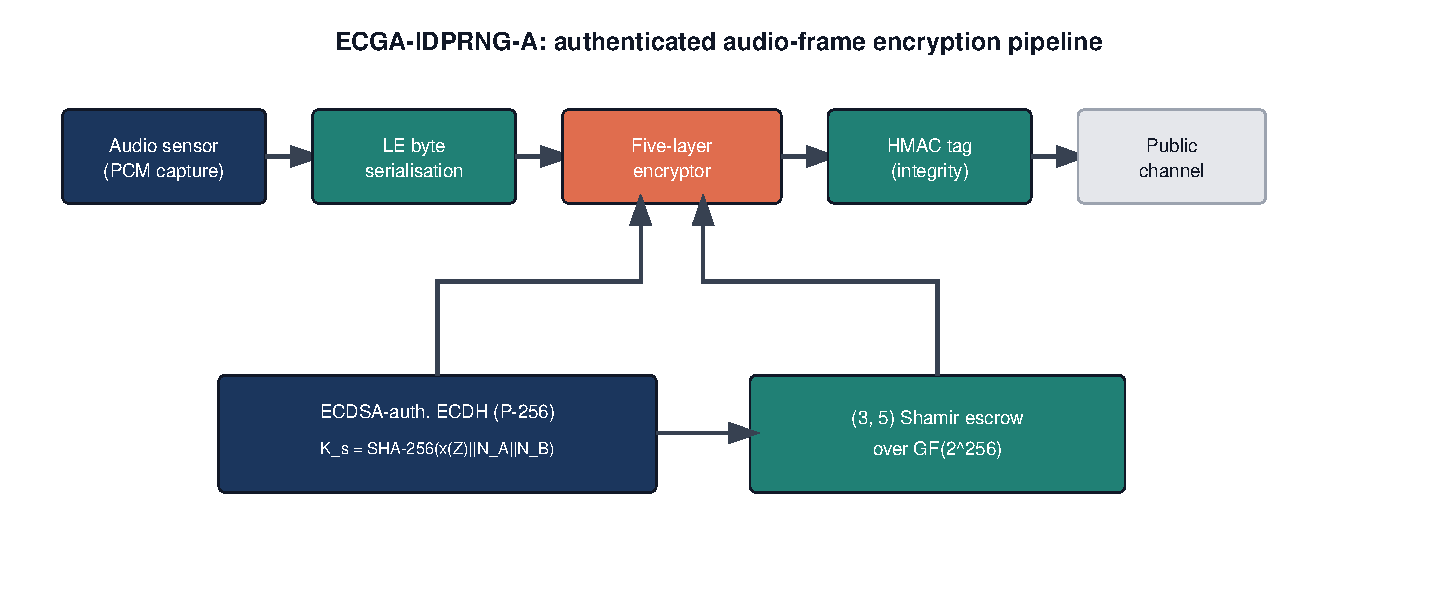
\includegraphics[width=0.9\linewidth]{paper3_audio_figures/fig1_arch.pdf}
\caption{Our end-to-end ECGA-IDPRNG-A architecture. Captured PCM audio is byte-serialised, encrypted by the five-layer core, authenticated with an HMAC tag, and sent over a public channel. The session key is established by an ECDSA-authenticated P-256 exchange and escrowed with a $(3,5)$ Shamir threshold scheme over $\mathrm{GF}(2^{256})$.}
    \label{fig:figarch}
\end{figure}

\begin{figure}[htbp]
\centering
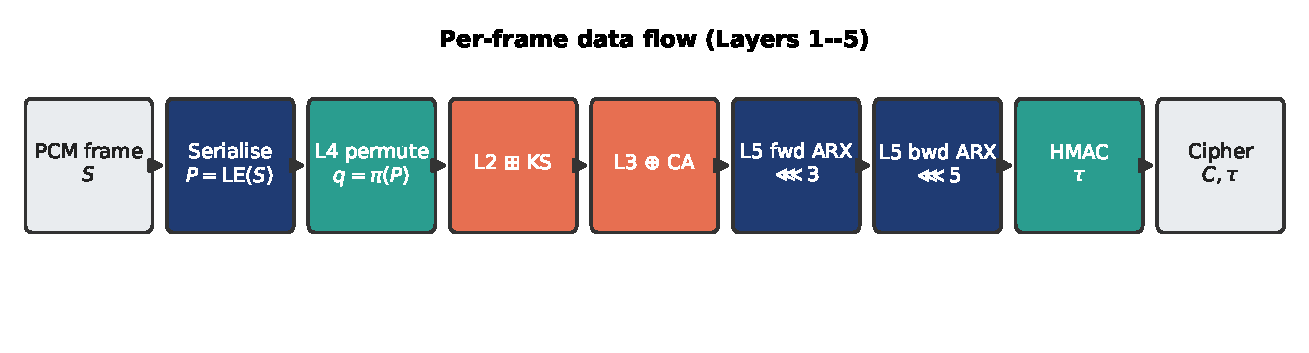
\includegraphics[width=\textwidth]{paper3_audio_figures/fig2_pipeline.pdf}
\caption{Per-frame data flow through Layers~1--5: little-endian serialisation, logistic byte permutation, modular keystream addition, Rule-30 mask XOR, the forward and backward ARX passes, and HMAC tagging.}
\label{fig:pipeline}
\end{figure}

\subsection{Layer 1: authenticated key agreement and escrow}
\label{sec:layer1}

Before audio encryption, the communicating endpoints (sender $A$ and receiver $B$) must agree on a shared secret that an eavesdropper cannot learn. They execute an ECDSA-authenticated P-256 handshake (Section~\ref{sec:ecdh}) to produce the master session key $K_s$. To ensure recoverability in the event of device compromise or loss, $K_s$ is immediately escrowed using the $(k,n)$ Shamir secret sharing scheme (Section~\ref{sec:shamir}). The escrow ecosystem connects $A$, $B$, and a set of independent, trusted storage entities known as custodians. Acting as the dealer, endpoint $A$ mathematically splits the key into $n$ distinct shares and distributes them securely to the $n$ custodians. Any quorum of $k$ custodians can jointly reconstruct the key if authorised, while any subset of $k-1$ or fewer custodians learns nothing about the secret~\cite{shamir1979}. For this implementation, the threshold parameters are concretely set to $(k,n)=(3,5)$. 

To prevent cross-layer key reuse, four domain-separated subkeys ($K_{\mathrm{hyper}}$, $K_{\mathrm{ca}}$, $K_{\mathrm{perm}}$, and $K_{\mathrm{mac}}$) are immediately derived from $K_s$ using specific labels. These four subkeys are kept strictly private within the endpoints and are never shared across the network. This ensures that a statistical bias in one cryptographic layer, however unlikely, cannot propagate to another. Throughout this exchange, only the ephemeral public points ($Q_A$ and $Q_B$), the nonces ($N_A$ and $N_B$), and the ECDSA signatures are transmitted publicly between party $A$ and party $B$. The ephemeral scalars ($n_A$ and $n_B$) remain strictly private to their respective owners, while the computed shared secret ($Z$) and the resulting master session key ($K_s$) are derived locally by both parties without ever being exposed. Algorithm~\ref{alg:ecdh} details the complete parameter definitions, the handshake sequence, the explicit subkey derivations, and the escrow distribution.

\begin{algorithm}[htbp]
\caption{Authenticated session-key agreement, subkey derivation, and $(k,n)$ threshold escrow}
\label{alg:ecdh}
\begin{algorithmic}[1]
\Require 
    \Statex \textbf{Static Public Parameters:} NIST P-256 curve generator $G$; long-term ECDSA public keys $pk_A, pk_B$; domain labels \texttt{"hyper"}, \texttt{"ca"}, \texttt{"perm"}, \texttt{"mac"}; frame length $L$; certified chaotic parameters $\theta^\ast$
    \Statex \textbf{Static Private Parameters:} Long-term ECDSA private signing keys $sk_A, sk_B$
    \Statex \textbf{Publicly Transmitted Variables:} Ephemeral points $Q_A, Q_B$; nonces $N_A, N_B$; signatures $\sigma_A, \sigma_B$
    \Statex \textbf{Strictly Private/Local Variables (Never Transmitted):} Ephemeral scalars $n_A, n_B$; shared point $Z$; master key $K_s$; subkeys $K_{\mathrm{hyper}}, K_{\mathrm{ca}}, K_{\mathrm{perm}}, K_{\mathrm{mac}}$
    \Statex \textbf{Entities:} Endpoints $A$ (Sender) and $B$ (Receiver); Custodians $C_1, \dots, C_n$ (independent storage nodes)
    \Statex \textbf{Threshold:} $(k,n)$ parameters over $\mathrm{GF}(2^{256})$, concretely $(3,5)$
\Ensure Domain-separated subkeys $K_{\mathrm{hyper}}, K_{\mathrm{ca}}, K_{\mathrm{perm}}, K_{\mathrm{mac}}$; shares $f(1),\dots,f(n)$
\State $A$: sample ephemeral scalar $n_A$ and nonce $N_A$; compute public point $Q_A=n_A G$
\State $A$: compute signature $\sigma_A = \mathrm{Sign}_{sk_A}(Q_A||N_A)$ and send $(Q_A, N_A, \sigma_A)$ to $B$
\State $B$: sample ephemeral scalar $n_B$ and nonce $N_B$; compute public point $Q_B=n_B G$
\State $B$: compute signature $\sigma_B = \mathrm{Sign}_{sk_B}(Q_B||N_B)$ and send $(Q_B, N_B, \sigma_B)$ to $A$
\State $A, B$: verify peer's signature using $pk_B$ and $pk_A$ respectively; \textbf{abort} if verification fails
\State $A, B$: compute shared secret point $Z \gets n_A Q_B = n_B Q_A$
\State $A, B$: form the canonical transcript $T \gets \mathrm{sort}\big(Q_A\|N_A,\; Q_B\|N_B\big)$ and $t \gets \mathrm{SHA\text{-}256}(T)$ \Comment{same order at both peers}
\State $A, B$: derive master session key $K_s \gets \mathrm{HKDF\text{-}SHA256}\big(x(Z);\ \mathrm{salt}=t;\ \mathrm{info}=\mathtt{"ECGA\text{-}IDPRNG\text{-}A/v2/session"}\big)$ and $\mathrm{session\_id} \gets t[0{:}16]$
\State $A, B$: derive $K_X \gets \mathrm{HKDF\text{-}SHA256}\big(K_s;\ \mathrm{info}=\mathtt{"ECGA\text{-}IDPRNG\text{-}A/v2/"}\|X\big)$ for $X \in \{\mathtt{hyper}, \mathtt{ca}, \mathtt{perm}, \mathtt{mac}\}$
\State $A$: sample random coefficients $r_1,\dots,r_{k-1} \in \mathrm{GF}(2^{256})$ uniformly at random
\State $A$: construct polynomial $f(x) = K_s + r_1x + \dots + r_{k-1}x^{k-1}$ over $\mathrm{GF}(2^{256})$
\State $A$: evaluate $f(x)$ to generate shares $f(1), \dots, f(n)$
\State $A$: distribute exactly one share $f(i)$ to each custodian $C_i$ via a secure channel
\State \Return Subkeys $(K_{\mathrm{hyper}}, K_{\mathrm{ca}}, K_{\mathrm{perm}}, K_{\mathrm{mac}})$ for Layers 2--5, and escrowed shares $\{f(i)\}_{i=1}^{n}$
\end{algorithmic}
\end{algorithm}

\subsection{Layer 2: Genetically certified hyperchaotic keystream}
\label{sec:layer2}

Every frame needs its own long sequence of pseudo-random bytes, called a \emph{keystream}, to mask the plaintext. Layer~2 generates this sequence from the four-dimensional hyperchaotic system of Equation~\eqref{eq:hyper}, seeded with the domain-separated subkey $K_{\mathrm{hyper}}$. The system is integrated numerically using a fourth-order Runge--Kutta method with step size $h=0.01$; the first $1000$ steps are discarded as warm-up so the trajectory settles onto the attractor. To prevent the state variables from growing without bound during a long phone call, each component is reduced modulo $1000$ using the $\mathrm{fmod}$ operation after every step. Each state component then yields one keystream byte by taking its fractional part (the digits after the decimal point), scaling it by $2^{32}$, and keeping the result modulo $256$:
\begin{equation}
\mathrm{KS}_i = \big\lfloor (|\xi_i| - \lfloor |\xi_i| \rfloor)\cdot 2^{32} \big\rfloor \bmod 256,
\label{eq:extract}
\end{equation}
where $\xi_i$ cycles through the four state variables in turn. The seed is the per-frame value $\kappa_{\mathrm{hyper}}=\mathrm{HMAC\text{-}SHA256}_{K_{\mathrm{hyper}}}(\texttt{"frame"}\|\mathrm{sid}\|\mathrm{ctr})$, so the keystream is fresh for every frame of a session. To obtain a stream that is indistinguishable from random even though the bare chaotic output fails some NIST tests (Table~\ref{tab:nist}), the chaotic bytes are XOR-combined with a SHAKE-256 extendable-output stream derived from the same seed; this whitening is what lets the confidentiality reduction (Theorem~\ref{thm:indcpa}) model Layer~2 as a secure PRG. The resulting keystream $\mathrm{KS}$ is passed as a primary cryptographic input to Layer~5. We note that the $\mathrm{fmod}\,1000$ reduction is applied to keep the trajectory bounded; it is a discontinuous wrap, so the certified Lyapunov exponent is understood as a property of the underlying flow.

The coefficients $(a,b,c,d,e)$ are not chosen by hand. Instead, a genetic algorithm searches for values that produce both statistically random-looking output and provably chaotic dynamics. Each candidate vector $\theta=(a,b,c,d,e)$ receives a fitness score
\begin{equation}
F(\theta) = w_1 H(\theta) + w_2\, \mathrm{NIST}(\theta) + w_3\, \lambda_1(\theta),
\label{eq:fitness}
\end{equation}
where $H$ measures byte entropy, $\mathrm{NIST}$ measures performance on a lightweight randomness test, and $\lambda_1$ is the largest Lyapunov exponent. We use weights $w_1 = w_2 = 1.0$ and $w_3 = 0.5$. The critical difference from prior work is that we do not merely reduce the fitness when $\lambda_1$ is small. We enforce
\begin{equation}
\lambda_1(\theta) > 0 \quad \text{as a hard admissibility constraint,}
\label{eq:constraint}
\end{equation}
which means any candidate whose largest Lyapunov exponent is zero or negative is discarded immediately, before its fitness is even calculated. A non-positive exponent signals that the system is not truly chaotic: it may be periodic or settling to a fixed point. For a long audio stream, even a brief excursion into such behaviour produces a run of correlated keystream bytes that could recreate audible formant bands in the ciphertext. By culling these candidates outright, we guarantee the deployed generator stays hyperchaotic for the entire session. The search uses a population of $50$, at most $100$ generations, crossover probability $0.8$, and Gaussian mutation with standard deviation $\sigma=0.01$. Convergence results are reported in Table~\ref{tab:ga} and Figure~\ref{fig:ga}.

\subsection{Layer 3: Rule-30 diffusion mask}
\label{sec:layer3}

Layer~3 adds an independent second source of randomness called a \emph{diffusion mask}. A ring of $512$ binary cells is seeded from the domain-separated subkey $K_{\mathrm{ca}}$ and evolved $512$ steps according to the Rule-30 update of Equation~\eqref{eq:rule30}. The successive cell states are packed into bytes to form a mask $\mathrm{CA}$ of the same length as the frame. Because this seed is derived from the session key, the mask is different for every session, yet deterministic for the receiver who holds the same key. The fully generated mask $\mathrm{CA}$ is given as output from this layer to serve as a secondary mixing variable for Layer~5.

\subsection{Layer 4: logistic byte permutation}
\label{sec:layer4}

Layer~4 shuffles the bytes using a permutation $\pi$ derived from the logistic map of Equation~\eqref{eq:logistic}. The map is iterated $50$ warm-up times from a seed derived from the domain-separated subkey $K_{\mathrm{perm}}$, then $L=2N$ successive values are recorded. Sorting these values into ascending order gives the permutation
\begin{equation}
\pi = \operatorname{argsort}(x_0,\dots,x_{L-1}),
\label{eq:perm}
\end{equation}
which tells us where each plaintext byte moves to in the shuffled block to produce the permuted bytes $q = \pi(P)$. The key point is that $\pi$ acts on \emph{bytes}, not on whole samples. A $16$-bit sample consists of a low byte and a high byte; the permutation separates these two bytes and places them far apart in the frame. This is what breaks the smooth amplitude trajectory responsible for the high adjacent-sample correlation seen in Table~\ref{tab:corr}. This permuted plaintext array $q$ is outputted as the foundational data input for Layer~5.

\subsection{Layer 5: two-pass ARX transform with authentication}
\label{sec:layer5}

The final layer mixes the permuted plaintext $q$ (from Layer~4) with the keystream $\mathrm{KS}$ (from Layer~2) and the diffusion mask $\mathrm{CA}$ (from Layer~3), guaranteeing that every output byte depends on every input byte. The \emph{forward pass} walks from the first byte to the last, mixing each byte with the keystream and the mask and then adding the result to a running total:
\begin{equation}
f_i = \big(((q_i \boxplus \mathrm{KS}_i) \oplus \mathrm{CA}_i) \lll 3\big) \boxplus f_{i-1}, \qquad f_{-1}=\texttt{0xA5},
\label{eq:fwd}
\end{equation}
for $i=0,\dots,L-1$. The \emph{backward pass} then walks from the last byte back to the first, propagating information in the reverse direction:
\begin{equation}
c_i = (f_i \boxplus c_{i+1}) \lll 5, \qquad c_L=\texttt{0x3C},
\label{eq:bwd}
\end{equation}
for $i=L-1,\dots,0$. The two passes together ensure that flipping a single bit in the original audio changes close to half the bits in the entire ciphertext frame (measured at $42.2\%$ in the worked example of Section~\ref{sec:worked}), a property called the \emph{avalanche effect}. The frame is then tagged for integrity using the final domain-separated subkey:
\begin{equation}
\tau = \mathrm{HMAC\text{-}SHA256}_{K_{\mathrm{mac}}}(C).
\label{eq:tag}
\end{equation}

Decryption performs the steps in reverse. The receiver first checks the tag $\tau$; if it does not match, the frame is discarded immediately. If it matches, the receiver applies a series of inverse mathematical operations:
\begin{equation}
P = \pi^{-1}\big(\mathsf{InvFwd}(\mathsf{InvBwd}(C))\big).
\label{eq:dec}
\end{equation}
Specifically, $\mathsf{InvBwd}(C)$ isolates the intermediate array $f$ by reversing the 5-bit cyclic shift and modular addition of Equation~\eqref{eq:bwd}, calculating $f_i = (c_i \ggg 5) \boxminus c_{i+1}$ sequentially from $i=0$ to $L-1$, where $\boxminus$ denotes subtraction modulo $256$. Next, $\mathsf{InvFwd}(f)$ recovers the permuted sequence $q$ by reversing the operations of Equation~\eqref{eq:fwd}, computing $q_i = \big(((f_i \boxminus f_{i-1}) \ggg 3) \oplus \mathrm{CA}_i\big) \boxminus \mathrm{KS}_i$. Finally, the inverse permutation $\pi^{-1}$ is applied to $q$ to perfectly reconstruct the original plaintext array $P$. Algorithm~\ref{alg:enc} details the complete programmatic procedure.

\begin{algorithm}[htbp]
\caption{Audio frame encryption (Layers 2--5)}
\label{alg:enc}
\begin{algorithmic}[1]
\Require
    \Statex \textbf{Static Public Parameters:} Frame length $L=2N$; certified chaotic parameters $\theta^\ast$; session identifier $\mathrm{sid}$; frame counter $\mathrm{ctr}\in[0,2^{64})$
    \Statex \textbf{Strictly Private/Local Inputs (Never Transmitted):} Serialised plaintext frame $P$; domain-separated subkeys $K_{\mathrm{hyper}}, K_{\mathrm{ca}}, K_{\mathrm{perm}}, K_{\mathrm{mac}}$
\Ensure Publicly transmitted $(\mathrm{ctr}, C, \tau)$
\State \textbf{for} $X\in\{\mathrm{hyper},\mathrm{ca},\mathrm{perm}\}$: $\ \kappa_X \gets \mathrm{HMAC\text{-}SHA256}_{K_X}(\mathtt{"frame"}\|\mathrm{sid}\|\mathrm{ctr})$ \Comment{per-frame seeds}
\State $\mathrm{KS} \gets \textsc{Keystream}(\kappa_{\mathrm{hyper}},\theta^\ast,L)$ \Comment{Eq.~\eqref{eq:extract}; whitened with SHAKE-256; state reduced $\bmod 1000$ after each RK4 step}
\State $\mathrm{CA} \gets \textsc{RuleThirtyMask}(\kappa_{\mathrm{ca}},L)$
\State $\pi \gets \textsc{LogisticPerm}(\kappa_{\mathrm{perm}},L)$
\State $q \gets \pi(P)$ \Comment{Permute plaintext bytes}
\State $f_{-1}\gets\texttt{0xA5}$
\For{$i=0$ to $L-1$}
  \State $f_i \gets (((q_i \boxplus \mathrm{KS}_i)\oplus \mathrm{CA}_i)\lll 3)\boxplus f_{i-1}$
\EndFor
\State $c_L\gets\texttt{0x3C}$
\For{$i=L-1$ down to $0$}
  \State $c_i \gets (f_i \boxplus c_{i+1})\lll 5$
\EndFor
\State $C \gets (c_0,\dots,c_{L-1})$
\State $\tau \gets \mathrm{HMAC\text{-}SHA256}_{K_{\mathrm{mac}}}(\mathrm{sid}\,\|\,\mathrm{ctr}\,\|\,|C|\,\|\,C)$ \Comment{Encrypt-then-MAC over counter and header}
\State \Return $\mathrm{ctr}, C,\tau$
\end{algorithmic}
\end{algorithm}


Algorithm~\ref{alg:dec} inverts the pipeline. It begins with strict authentication: the receiver recomputes the HMAC tag $\tau'$ over the session identifier, counter and ciphertext with $K_{\mathrm{mac}}$ and compares it to $\tau$ in constant time, rejecting the frame before any decryption if they differ (or if the counter is not strictly increasing). When the session key was reconstructed from escrow custodians, this same check verifies the gathered shares: an invalid combination yields a wrong $K_{\mathrm{mac}}$ and fails the tag.

Once the frame is authenticated, the receiver uses the remaining domain-separated subkeys to deterministically regenerate the cryptographic states used during encryption. Each subkey serves a specific, isolated role: $K_{\mathrm{hyper}}$ seeds the hyperchaotic system to generate the primary masking keystream ($\mathrm{KS}$), $K_{\mathrm{ca}}$ seeds the Rule-30 cellular automaton to generate a secondary spatial diffusion mask ($\mathrm{CA}$), and $K_{\mathrm{perm}}$ seeds the logistic map to create the permutation vector ($\pi$) responsible for destroying the audio's temporal correlation. Deriving independent subkeys from the master session key ensures that a statistical bias in one generator cannot propagate to or compromise the others.

With the cryptographic states regenerated, the two-pass ARX transform is unwound in reverse order. The inverse backward pass recovers the intermediate array $f$ by applying a 5-bit right cyclic shift and modular subtraction. The inverse forward pass then isolates the permuted plaintext array $q$ by unwinding the XOR diffusion mask and subtracting the hyperchaotic keystream modulo 256. Finally, the receiver applies the inverse permutation mapping $\pi^{-1}$ to $q$, restoring the original byte ordering to yield the plaintext byte array $P$. These little-endian bytes are packed back together ($p_{2j} + (p_{2j+1} \ll 8)$) to perfectly reconstruct the original 16-bit signed PCM audio samples $S$.

\begin{algorithm}[!ht]
\caption{Audio frame decryption and signal reconstruction (Inverse Layers 5--2)}
\label{alg:dec}
\begin{algorithmic}[1]
\Require Received $(\mathrm{ctr}, C, \tau)$; session identifier $\mathrm{sid}$; domain-separated subkeys $(K_{\mathrm{hyper}}, K_{\mathrm{ca}}, K_{\mathrm{perm}}, K_{\mathrm{mac}})$; certified $\theta^\ast$; last accepted counter $\mathrm{ctr}_{\mathrm{last}}$
\Ensure Reconstructed plaintext byte array $P$; recovered PCM audio samples $S = (s_0,\dots,s_{N-1})$
\If{$\mathrm{ctr} \le \mathrm{ctr}_{\mathrm{last}}$} \State \textbf{abort} \Comment{Reject replayed/reordered frame} \EndIf
\State $\tau' \gets \mathrm{HMAC\text{-}SHA256}_{K_{\mathrm{mac}}}(\mathrm{sid}\,\|\,\mathrm{ctr}\,\|\,|C|\,\|\,C)$ \Comment{Authenticate frame integrity}
\If{$\tau' \neq \tau$}
    \State \textbf{abort} \Comment{Reject tampered or corrupted frame immediately}
\EndIf
\State \textbf{for} $X\in\{\mathrm{hyper},\mathrm{ca},\mathrm{perm}\}$: $\ \kappa_X \gets \mathrm{HMAC\text{-}SHA256}_{K_X}(\mathtt{"frame"}\|\mathrm{sid}\|\mathrm{ctr})$
\State $\mathrm{KS} \gets \textsc{Keystream}(\kappa_{\mathrm{hyper}},\theta^\ast,L)$ \Comment{Regenerate identical whitened keystream}
\State $\mathrm{CA} \gets \textsc{RuleThirtyMask}(\kappa_{\mathrm{ca}},L)$ \Comment{Regenerate cellular automaton diffusion mask}
\State $\pi \gets \textsc{LogisticPerm}(\kappa_{\mathrm{perm}},L)$ \Comment{Regenerate permutation vector}
\State Compute inverse permutation mapping $\pi^{-1}$
\State $c_L \gets \texttt{0x3C}$
\For{$i = 0$ to $L-1$} \Comment{Inverse backward ARX pass}
    \State $f_i \gets ((c_i \ggg 5) \boxminus c_{i+1}) \bmod 256$
\EndFor
\State $f_{-1} \gets \texttt{0xA5}$
\For{$i = 0$ to $L-1$} \Comment{Inverse forward ARX pass}
    \State $t_i \gets (f_i \boxminus f_{i-1}) \bmod 256$
    \State $q_i \gets (((t_i \ggg 3) \oplus \mathrm{CA}_i) \boxminus \mathrm{KS}_i) \bmod 256$
\EndFor
\State $P \gets \pi^{-1}(q)$ \Comment{Reverse logistic permutation to restore byte ordering}
\For{$j = 0$ to $N-1$} \Comment{Reconstruct 16-bit signed PCM audio samples}
    \State $s_j \gets p_{2j} + (p_{2j+1} \ll 8)$
\EndFor
\State \Return $P, S$
\end{algorithmic}
\end{algorithm}

\subsection{Active-stream Lyapunov monitor}
\label{sec:asl}

A phone call or audio feed can last for hours, which is much longer than the short tests used during the genetic setup. Over such a long time, even a certified hyperchaotic system might drift into a weak state due to numerical rounding errors. To prevent this, an \emph{active-stream Lyapunov (ASL) monitor} continuously watches the generator while the session is live. It regularly calculates the local divergence rate (how fast two close points separate) directly from the keystream bytes being produced. If this rate drops near zero, it is a clear indication that the system is about to lose its chaotic behaviour. To fix this, the monitor immediately triggers a new key-agreement handshake \emph{before} the weak keystream can be used. This ensures that the strict positive Lyapunov rule enforced during the initial design is also maintained in real time, protecting long continuous audio streams instead of just single frames.

\section{Worked Example}
\label{sec:worked}

To show that the pipeline is fully reproducible, we now encrypt a frame of eight $16$-bit PCM samples by hand, following the five layers of Section~\ref{sec:framework} in order. The eight samples are
\begin{equation}
S = (1200,\,-3400,\,15000,\,-800,\,25,\,32000,\,-16000,\,5000).
\label{eq:sample_values}
\end{equation}
To make this numerical example fully reproducible without requiring the reader to compute elliptic-curve point multiplications by hand, we simulate the key-agreement phase. Equation~\eqref{eq:sessionkey} uses $x(Z)$, which represents the $x$-coordinate of the shared elliptic curve secret. For this demonstration, we replace the $x(Z)$ value with a deterministic ASCII prefix \texttt{"ECGA-IDPRNG-A::demo"}. This prefix is then appended with the segments \texttt{"NA=7b1e"} and \texttt{"NB=d92a"}, joined by the separator \texttt{"::"}; these segments simulate the hexadecimal nonces $N_A$ and $N_B$ exchanged during the handshake. We derive the session key $K_s$ by hashing this complete combined string,
\begin{equation*}
K_s = \mathrm{SHA\text{-}256}(\texttt{"ECGA-IDPRNG-A::demo::NA=7b1e::NB=d92a"}).
\end{equation*}
Evaluating this hash produces a fixed 256-bit session key whose first four bytes are \texttt{16\,97\,fa\,c7} in hexadecimal. This deterministic generation allows any reader to independently reproduce the exact subkeys, keystream, and ciphertext arrays shown below.

\subsection{Step 1: byte serialisation}

The cipher uses the samples as raw bytes in \emph{little-endian} format, wherein each $16$-bit sample is split into two bytes: the low byte (the remainder after dividing by $256$) comes first, and the high byte (the quotient after dividing by $256$) comes second. For example, sample $s_0=1200$ in hexadecimal is $\texttt{0x04B0}$. The low byte is $\texttt{0xB0}=176$ and the high byte is $\texttt{0x04}=4$, so the pair is $(176,4)$.

Applying this to all eight samples of Equation~\eqref{eq:sample_values}, following Equation~\eqref{eq:serial}, yields $L=16$ bytes. We show them row-major as a $4\times4$ block:
\begin{equation*}
P=\begin{bmatrix}176&4&184&242\\152&58&224&252\\25&0&0&125\\128&193&136&19\end{bmatrix}.
\end{equation*}
Sample $s_0=1200=\texttt{0x04B0}$ appears as $(176,4)$ in the first row; $s_1=-3400=\texttt{0xF2B8}$ appears as $(184,242)$; and so on. This byte array $P$ is what actually enters the cipher.

\subsection{Step 2: keystream and diffusion mask}

Layer~2 produces a keystream $\mathrm{KS}$ of $16$ pseudo-random bytes from the hyperchaotic generator, and Layer~3 produces a diffusion mask $\mathrm{CA}$ of $16$ bytes from the Rule-30 automaton. Both are seeded from the same $K_s$, so they are deterministic for anyone who holds the key. For this frame they are:
\begin{equation*}
\mathrm{KS}=\begin{bmatrix}218&207&224&138\\13&13&185&189\\246&119&147&42\\6&136&200&181\end{bmatrix},\qquad
\mathrm{CA}=\begin{bmatrix}209&44&52&60\\72&88&73&103\\12&24&171&38\\91&4&246&163\end{bmatrix}.
\end{equation*}
These bytes will be mixed with the plaintext bytes in the ARX transform.

\subsection{Step 3: byte permutation}

Layer~4 uses the logistic map to decide a shuffling order. Sorting $16$ map values into ascending order gives the permutation
\begin{equation*}
\pi=(9,10,11,0,12,1,6,13,2,7,4,14,15,3,5,8).
\end{equation*}
This means: the byte placed at position $i$ in $Q$ comes from position $\pi(i)$ in $P$; for example, position $0$ of $Q$ receives the byte from position $9$ of $P$, position $1$ of $Q$ receives the byte from position $10$ of $P$, and so on. Applying $\pi$ to the $16$ bytes of $P$ gives the permuted block
\begin{equation*}
Q=\pi(P)=\begin{bmatrix}0&0&125&176\\128&4&224&193\\184&252&152&136\\19&242&58&25\end{bmatrix}.
\end{equation*}
Notice how the low and high bytes of the original samples are now scattered: the $176$ from $s_0$ sits next to the $125$ from $s_3$, breaking the smooth waveform shape.

\subsection{Step 4: forward ARX pass}

Layer~5 first runs a forward pass that mixes information from left to right. For each byte position $i$, we compute:
\begin{enumerate}
\item Add the plaintext byte to the keystream byte, modulo $256$ (wrap around if the sum exceeds $255$).
\item XOR the result with the diffusion-mask byte.
\item Rotate the resulting byte left by $3$ bit positions.
\item Add this to the previous forward value $f_{i-1}$, modulo $256$.
\end{enumerate}
The chain starts with $f_{-1}=\texttt{0xA5}=165$. Table~\ref{tab:fwd} shows every intermediate value for all $16$ positions.

\begin{table}[htbp]
\centering
\caption{Forward ARX pass. Columns follow Eq.~\eqref{eq:fwd}: the modular sum $q_i\boxplus\mathrm{KS}_i$, the XOR with the diffusion mask, the left rotation by $3$, and the accumulated $f_i$.}
\label{tab:fwd}
\small
\begin{tabular}{cccccccc}
\toprule
$i$ & $Q_i$ & $\mathrm{KS}_i$ & $\mathrm{CA}_i$ & $Q_i\boxplus\mathrm{KS}_i$ & $\oplus\,\mathrm{CA}_i$ & $\lll 3$ & $f_i$ \\
\midrule
0 & 0 & 218 & 209 & 218 & 11 & 88 & 253 \\
1 & 0 & 207 & 44 & 207 & 227 & 31 & 28 \\
2 & 125 & 224 & 52 & 93 & 105 & 75 & 103 \\
3 & 176 & 138 & 60 & 58 & 6 & 48 & 151 \\
4 & 128 & 13 & 72 & 141 & 197 & 46 & 197 \\
5 & 4 & 13 & 88 & 17 & 73 & 74 & 15 \\
6 & 224 & 185 & 73 & 153 & 208 & 134 & 149 \\
7 & 193 & 189 & 103 & 126 & 25 & 200 & 93 \\
8 & 184 & 246 & 12 & 174 & 162 & 21 & 114 \\
9 & 252 & 119 & 24 & 115 & 107 & 91 & 205 \\
10 & 152 & 147 & 171 & 43 & 128 & 4 & 209 \\
11 & 136 & 42 & 38 & 178 & 148 & 164 & 117 \\
12 & 19 & 6 & 91 & 25 & 66 & 18 & 135 \\
13 & 242 & 136 & 4 & 122 & 126 & 243 & 122 \\
14 & 58 & 200 & 246 & 2 & 244 & 167 & 33 \\
15 & 25 & 181 & 163 & 206 & 109 & 107 & 140 \\
\bottomrule
\end{tabular}
\end{table}

For example, at $i=0$: $Q_0=0$ plus $\mathrm{KS}_0=218$ gives $218$; XOR with $\mathrm{CA}_0=209$ gives $11$; rotate left by $3$ gives $88$; add to $f_{-1}=165$ gives $253$. The next position uses $f_0=253$ as its input, so every value depends on everything before it.

\subsection{Step 5: backward ARX pass}

The backward pass now mixes information from right to left. For each position $i$ (counting downward from $15$ to $0$), we add the forward value $f_i$ to the next ciphertext byte $c_{i+1}$, modulo $256$, and rotate the result left by $5$ bit positions. The chain starts with $c_{16}=\texttt{0x3C}=60$. Table~\ref{tab:bwd} gives the full trace.

\begin{table}[htbp]
\centering
\caption{Backward ARX pass, following Eq.~\eqref{eq:bwd}: each $c_i$ adds the successor ciphertext byte to $f_i$ and rotates left by $5$.}
\label{tab:bwd}
\small
\begin{tabular}{cccc}
\toprule
$i$ & $f_i$ & $f_i\boxplus c_{i+1}$ & $c_i$ \\
\midrule
0 & 253 & 61 & 167 \\
1 & 28 & 2 & 64 \\
2 & 103 & 55 & 230 \\
3 & 151 & 134 & 208 \\
4 & 197 & 127 & 239 \\
5 & 15 & 213 & 186 \\
6 & 149 & 54 & 198 \\
7 & 93 & 13 & 161 \\
8 & 114 & 133 & 176 \\
9 & 205 & 152 & 19 \\
10 & 209 & 94 & 203 \\
11 & 117 & 108 & 141 \\
12 & 135 & 191 & 247 \\
13 & 122 & 193 & 56 \\
14 & 33 & 58 & 71 \\
15 & 140 & 200 & 25 \\
\bottomrule
\end{tabular}
\end{table}

For example, at $i=15$: $f_{15}=140$ plus $c_{16}=60$ gives $200$; rotate left by $5$ gives $25$. At $i=14$: $f_{14}=33$ plus $c_{15}=25$ gives $58$; rotate left by $5$ gives $71$.

\subsection{Final ciphertext}

The resulting ciphertext bytes are
\begin{equation*}
C=\begin{bmatrix}167&64&230&208\\239&186&198&161\\176&19&203&141\\247&56&71&25\end{bmatrix}.
\end{equation*}
If these bytes are (meaninglessly) reinterpreted as little-endian $16$-bit PCM sample values, they read
\begin{equation*}
C_{\mathrm{pcm}} = (16551,\,-12058,\,-17681,\,-24122,\,5040,\,-29237,\,14583,\,6471),
\end{equation*}
which bears no resemblance to the original $S$. We stress that $C_{\mathrm{pcm}}$ is \emph{not} an audio signal: it is ciphertext viewed as numbers, with no acoustic meaning, and is shown only to illustrate how completely the original sample values are destroyed.

\subsection{Decryption}

The receiver first verifies the HMAC tag $\tau$ attached to the frame. If the tag is invalid, the frame is discarded. If it is valid, the receiver applies the inverse operations in reverse order: invert the backward pass of Equation~\eqref{eq:bwd}, invert the forward pass of Equation~\eqref{eq:fwd}, and finally apply the inverse permutation $\pi^{-1}$. This recovers $P$ exactly, and hence the original samples $S=(1200,-3400,15000,-800,25,32000,-16000,5000)$ bit-for-bit.

\subsection{Avalanche effect}

A good cipher must spread a tiny change across the entire output. To test this, we flipped the least-significant bit of the first sample (changing $1200$ to $1201$) and re-encrypted. The resulting ciphertext differed in $15$ of the $16$ bytes and in $54$ of the $128$ ciphertext bits ($42.2\%$, very close to the ideal $50\%$). The single unchanged byte is a coincidental $8$-bit value collision, not a structural weakness. This near-complete diffusion is caused by the two chained passes of Equations~\eqref{eq:fwd} and~\eqref{eq:bwd}: a one-bit change in one sample propagates through the forward chain, then through the backward chain, affecting essentially every byte in the frame.

\section{Security Analysis}
\label{sec:security}

This section proves that the scheme meets the five goals stated in Section~\ref{sec:threat}. We first demonstrate that the encrypted frames successfully hide their content (confidentiality), then verify that tampering is detected (integrity), and finally confirm that the session key is agreed upon securely and remains recoverable by an authorised quorum. We establish these properties through standard cryptographic reductions, bounding the success of any computationally bounded adversary against well-studied hardness assumptions.

\subsection{Confidentiality}

Our first theorem establishes that an adversary observing a ciphertext cannot determine which of two candidate audio frames was encrypted. This aligns with the formal definition of confidentiality, known as indistinguishability under chosen-plaintext attack (IND-CPA).

\begin{theorem}[IND-CPA]
\label{thm:indcpa}
Model the whitened Layer~2 keystream generator (the hyperchaotic bytes XOR-combined with a SHAKE-256 output, Remark~\ref{rem:scope}) as a pseudo-random generator $G$, and $\mathrm{HMAC\text{-}SHA256}$ as a random oracle $H$. Assume each frame uses a distinct counter $\mathrm{ctr}$ under one session key, so no two frames reuse the same keystream. For every probabilistic polynomial-time adversary $\mathcal{A}$ against the frame scheme $\Pi$ making at most $q_H$ oracle queries there exist adversaries $\mathcal{B},\mathcal{B}'$ of essentially the same running time with
\[
\mathrm{Adv}^{\mathrm{cpa}}_{\Pi}(\mathcal{A}) \;\le\; \mathrm{Adv}^{\mathrm{prg}}_{G}(\mathcal{B}) + \frac{q_H}{2^{256}}.
\]
\end{theorem}

Informally, this theorem establishes that if the hyperchaotic keystream is indistinguishable from a truly random byte sequence, and if the HMAC behaves as an ideal random function, no computationally bounded attacker can distinguish between encrypted frames significantly better than random chance. The adversary's advantage is strictly bounded by two negligible quantities: their ability to distinguish the hyperchaotic generator's output from true randomness, and the probability of accidentally guessing the 256-bit session key during a MAC query.

\begin{proof}
We construct a sequence of three hybrid experiments, or \emph{games}. In each game, the adversary $\mathcal{A}$ attempts to guess a secret challenge bit, and we demonstrate that their probability of success changes by only a negligible margin between successive games. Let $\mathrm{Win}_j$ denote the event that $\mathcal{A}$ guesses the challenge bit correctly in Game~$j$.

\emph{Game 0} is the real IND-CPA experiment from Definition~\ref{def:indcpa}. The challenger serialises the chosen audio frame into bytes, applies the certified keystream $\mathrm{KS}$, the diffusion mask $\mathrm{CA}$, the permutation $\pi$, and the two ARX passes, ultimately returning the ciphertext and its HMAC tag. By definition, the probability that $\mathcal{A}$ wins this game is $\Pr[\mathrm{Win}_0]=\tfrac12+\mathrm{Adv}^{\mathrm{cpa}}_{\Pi}(\mathcal{A})$.

\emph{Game 1} is identical to Game~0, except that the keystream bytes $\mathrm{KS}_i$ used in the forward pass of Equation~\eqref{eq:fwd} are replaced by truly random bytes drawn from a uniform distribution. If the attacker behaves differently in Game~1 than in Game~0, that difference directly translates to an ability to distinguish the hyperchaotic generator from true randomness. We therefore construct a reduction adversary $\mathcal{B}$ that exploits this difference: $\mathcal{B}$ receives a string of bytes (either from the real generator or from a random source), injects them into the encryption procedure in place of $\mathrm{KS}$, and outputs whatever $\mathcal{A}$ outputs. By construction, the advantage of $\mathcal{B}$ in distinguishing the generator equals the difference in $\mathcal{A}$'s success rate between the two games. Hence, $|\Pr[\mathrm{Win}_1]-\Pr[\mathrm{Win}_0]|\le \mathrm{Adv}^{\mathrm{prg}}_{G}(\mathcal{B})$.

\emph{Game 2} modifies Game~1 by answering every HMAC tag query with a fresh random 256-bit string. The challenger maintains a lookup table to ensure consistent responses if the same message is queried multiple times. The only scenario where the attacker can distinguish Game~2 from Game~1 is by querying the random oracle $H$ using the exact secret session key. Because the session key is 256 bits long, each of the $q_H$ queries has a maximum probability of $2^{-256}$ of hitting this exact string. Therefore, $|\Pr[\mathrm{Win}_2]-\Pr[\mathrm{Win}_1]|\le q_H/2^{256}$.

In Game~2, the forward pass adds a uniform, independent random byte to each permuted plaintext byte before any further operation. Adding a uniformly random byte modulo $256$ is mathematically equivalent to applying a one-time pad: the result is statistically independent of the original plaintext byte. Consequently, the intermediate values $f_i$, and the final ciphertext (which is a strictly invertible function of $f_i$ and the random tag), are distributed independently of the underlying audio frame. The attacker gains no information, reducing their optimal strategy to random guessing, which yields $\Pr[\mathrm{Win}_2]=\tfrac12$.

Summing these bounds directly yields the theorem statement.
\end{proof}

\begin{remark}[Scope of the guarantee]
\label{rem:scope}
The reduction in Theorem~\ref{thm:indcpa} is \emph{conditional}: the security of the audio encryption is only as strong as the pseudo-randomness of the Layer~2 keystream. We stress that this assumption is placed on the \emph{whitened} generator. The bare chaotic stream fails the NIST monobit, DFT and Maurer tests (Table~\ref{tab:nist}) and is therefore efficiently distinguishable from random, so it cannot by itself be modelled as a secure PRG; a positive Lyapunov exponent is a property of the continuous dynamics and does not imply cryptographic pseudo-randomness. We therefore pass the chaotic bytes through a NIST-standard extendable-output function (SHAKE-256), after which the PRG assumption rests on a standard primitive and the chaotic system acts as a seed-mixing source. This matters greatly for a live audio feed. A telephone call does not encrypt one frame but hundreds or thousands; the per-frame counter makes each frame's keystream independent, and the assumption is that the whitened generator remains indistinguishable from random for the entire duration of the call.

This is exactly why the scheme includes two further safeguards. First, the genetic search enforces a strictly positive largest Lyapunov exponent (Equation~\eqref{eq:constraint}), eliminating parameter vectors that could ever collapse into periodic behaviour. Second, the active-stream Lyapunov monitor of Section~\ref{sec:asl} watches the generator at run time and triggers re-keying if the local divergence rate drops. Together these mechanisms ensure that the premise of the theorem---that the generator stays unpredictable---remains true as the stream lengthens, so the confidentiality bound holds across the whole session and not merely at its beginning.
\end{remark}

\subsection{Integrity and key agreement}

\begin{theorem}[Ciphertext integrity]
\label{thm:int}
If $\mathrm{HMAC\text{-}SHA256}$ is an existentially unforgeable MAC, then no polynomial-time adversary can produce a novel frame $(C^\ast,\tau^\ast)$ consisting of an arbitrary tampered ciphertext $C^\ast$ and a purported authentication tag $\tau^\ast$ that was not generated by the sender yet passes verification, except with negligible probability.
\end{theorem}

\begin{proof}
When the receiver gets a potentially tampered frame $(\mathrm{ctr}^\ast, C^\ast,\tau^\ast)$, the very first step is to compute $\mathrm{HMAC\text{-}SHA256}_{K_{\mathrm{mac}}}(\mathrm{sid}\,\|\,\mathrm{ctr}^\ast\,\|\,|C^\ast|\,\|\,C^\ast)$ and compare it with $\tau^\ast$ in constant time. If the two match but the sender never produced this exact pair, then the attacker has forged an HMAC tag for a message they did not create---an \emph{existential forgery}. By assumption, HMAC-SHA256 is secure against such forgeries: success is negligible for any attacker who does not know $K_{\mathrm{mac}}$. Because the tag binds the session identifier and the per-frame counter, a replayed or reordered frame (a valid old $(C,\tau)$ presented under a different $\mathrm{ctr}$) also fails verification; the receiver additionally rejects any counter not strictly greater than the last accepted one. Since the tag is checked \emph{before} any decryption, a modified, forged, or replayed frame is rejected immediately and can never influence the recovered audio. This Encrypt-then-MAC composition~\cite{bellare2000} is what lifts the IND-CPA guarantee of Theorem~\ref{thm:indcpa} toward chosen-ciphertext security.
\end{proof}

\begin{remark}[CCA handling]
Although HMAC verification prior to decryption prevents typical chosen-ciphertext attacks in practice, we state only IND-CPA security formally to isolate the confidentiality of the core encryption layers. Upgrading to IND-CCA security is achieved straightforwardly via our Encrypt-then-MAC composition, but we leave the formal CCA reduction as a minor extension of Theorem~\ref{thm:indcpa}.
\end{remark}

\begin{theorem}[Authenticated key exchange]
\label{thm:ake}
Under the elliptic-curve computational Diffie--Hellman assumption on P-256 and the unforgeability of ECDSA, the handshake of Algorithm~\ref{alg:ecdh} yields a session key indistinguishable from random to any active adversary who does not hold a long-term signing key.
\end{theorem}

\begin{proof}
Each ephemeral public point ($Q_A$ or $Q_B$) is transmitted together with an ECDSA signature created using the sender's long-term private key. If an adversary tries to inject a fake point or alter an existing one, the signature verification on the receiving side will fail, because forging an ECDSA signature without the private key is assumed to be computationally infeasible. Therefore both endpoints receive each other's authentic ephemeral points.

With authentic points in hand, both endpoints compute the same shared point $Z=n_An_BG$. The \emph{computational Diffie--Hellman (CDH) assumption} says that given only the public points $Q_A$ and $Q_B$, no efficient algorithm can compute $x(Z)$, the $x$-coordinate of this shared point. Finally, the session key is $K_s=\mathrm{SHA\text{-}256}(x(Z)\|N_A\|N_B)$. Because $x(Z)$ is unknown to the attacker and the nonces $N_A,N_B$ are fresh, the output of SHA-256 is uniformly random from the attacker's point of view.
\end{proof}

\begin{theorem}[Forward secrecy]
\label{thm:fs}
Since the Diffie--Hellman exponents $n_A,n_B$ are ephemeral and erased after each session, disclosure of the long-term signing keys does not enable recovery of any prior session key.
\end{theorem}

\begin{proof}
The session key $K_s$ depends only on the ephemeral shared secret $n_An_BG$ and the nonces. The long-term ECDSA keys are used solely to \emph{authenticate} the handshake; they never enter the key-derivation hash. Once the ephemeral scalars $n_A$ and $n_B$ are erased from memory, the only way to recover $Z$ from the recorded transcript is to solve the CDH problem on P-256, which is assumed to be hard. Therefore, compromising the long-term signing keys---or even one session's ephemeral key---does not expose any other session.
\end{proof}

\begin{remark}[Escrow and forward secrecy]
Forward secrecy (Theorem~\ref{thm:fs}) holds provided the ephemeral DH exponents are erased and the Shamir shares are deleted by the custodians after the session ends. Retained shares would allow retrospective key reconstruction, breaking forward secrecy.
\end{remark}

\begin{theorem}[Threshold recovery]
\label{thm:share}
The $(k,n)$ sharing of Equation~\eqref{eq:share} allows any quorum of $k$ custodians to reconstruct $K_s$, while any subset of $k-1$ custodians obtains no information about it~\cite{shamir1979}. For our specific configuration of $(k,n)=(3,5)$, any three custodians can recover the key, while any two learn nothing.
\end{theorem}

\begin{proof}
The $n$ shares are evaluations of a degree-$(k-1)$ polynomial $f(x)$ over $\mathrm{GF}(2^{256})$, and the constant term of this polynomial is the secret $K_s$. A fundamental fact about polynomials is that any $k$ points determine a unique degree-$(k-1)$ polynomial, while $k-1$ points leave it completely undetermined. For example, with $k=3$, three shares determine $f(x)$ uniquely via Lagrange interpolation, and evaluating at $x=0$ recovers $f(0)=K_s$.

Conversely, consider an adversary who compromises strictly fewer than $k$ shares. In the specific case of our $(3,5)$ threshold where the adversary holds only two shares, $f(i)$ and $f(j)$, the secret remains unconditionally protected. For any arbitrary candidate value of the session key $K_s'$, there exists exactly one valid degree-two polynomial that simultaneously interpolates the known points $(i, f(i))$ and $(j, f(j))$ while possessing $K_s'$ as its constant term. Because every potential key in the finite field maps to a valid polynomial with equal probability, possessing only two shares yields zero information-theoretic advantage regarding the true secret. This perfect statistical independence strictly satisfies Assumption~\ref{as:escrow}.
\end{proof}

\subsection{Resistance to concrete attacks}

The experimental results in Section~\ref{sec:experiments} confirm that the scheme resists the standard families of cryptanalytic attack:

\begin{itemize}[leftmargin=2em]
\item \emph{Statistical attacks} exploit non-uniform byte distributions. They are defeated because the ciphertext byte histogram is flat and the Shannon entropy is near the maximum of 8 bits per byte (Table~\ref{tab:entropy}).

\item \emph{Spectral and intelligibility attacks} are the audio-specific threat identified in Section~\ref{sec:redundancy}. An attacker might try to read formant bands directly from the ciphertext spectrogram. These attacks are defeated because the spectral entropy collapses to near 1 and the spectral flatness rises to the white-noise floor (Table~\ref{tab:spectral}), leaving no coherent bands for a speech recogniser to exploit.

\item \emph{Correlation attacks} exploit the fact that adjacent samples in natural speech are highly correlated. They are defeated because the ciphertext adjacent-sample correlation drops to within $\pm0.014$ of zero (Table~\ref{tab:corr}).

\item \emph{Differential attacks} measure how much the ciphertext changes when the plaintext or key is altered slightly. Near-ideal NSCR and UACI values (Table~\ref{tab:diff}) show that a one-bit change in either the plaintext or the key propagates to essentially the entire ciphertext frame, giving the attacker no local structure to exploit.

\item \emph{Brute-force attacks} try every possible key. The session key occupies a $2^{256}$ space, while the overall security level is about $128$ bits, set by the P-256 elliptic curve (Pollard rho), as quantified below---far beyond any feasible search.
\end{itemize}

\subsection{Key space}
\label{sec:keyspace}

The confidentiality of every frame rests on the $256$-bit session key $K_s$ produced by Equation~\eqref{eq:sessionkey}. A direct brute-force search over $K_s$ spans $2^{256}$ keys. However, $K_s$ is agreed over the NIST P-256 curve, whose best known attack (Pollard rho) costs about $2^{128}$ operations, so the \emph{effective} security level is approximately $128$ bits---still far beyond any feasible computation.

The certified hyperchaotic parameter vector $\theta^\ast=(a,b,c,d,e)$ is \emph{not} a secret. It is a public constant of the cipher, published once after the genetic search finishes, and it is the same for every user and every session. An attacker does not need to guess $\theta^\ast$ because it is already known. It therefore contributes no additional entropy to the attacker's search. We make no claim of a key space larger than $2^{256}$; the effective security level is that of the underlying P-256 session key, about $128$ bits.

\section{Experimental Evaluation}
\label{sec:experiments}

This section reports every measurement that was performed to validate the scheme. We begin with the test setup, then examine the keystream quality, the genetic search convergence, the byte-level statistics, the spectral results (which are the central claim of the paper), the intelligibility collapse, the correlation destruction, the differential sensitivity, the error behaviour, the throughput, and finally a comparison with prior work. Every metric is reported per clip and as a mean~$\pm$~standard deviation across the full set of eight clips.

\subsection{Datasets and experimental protocol}
\label{sec:datasets}

\subsubsection{Procedural synthetic test signals}
In addition to standard corpora, we generate eight procedurally defined audio 
clips designed to stress-test specific spectral characteristics that an audio 
cipher must destroy. Each clip is 2~seconds long, mono, 16-bit PCM, sampled at 
8~kHz ($N=16000$ samples, $L=32000$ bytes per frame). Table~\ref{tab:synthetic_clips} 
summarises their design.

\begin{table}[t]
\centering
\caption{Procedural synthetic test clips. Each clip is 2~s, mono, 16-bit PCM at 8~kHz.}
\label{tab:synthetic_clips}
\begin{tabular}{@{}clp{5.5cm}l@{}}
\toprule
ID & Description & Spectral characteristic & Purpose \\
\midrule
S1 & Multi-formant speech-like & Energy at 500, 1500, 2500~Hz & Formant leakage test \\
S2 & Sustained musical chord & Multiple harmonic series & Harmonic structure test \\
S3 & Pure tone & Single frequency (1~kHz) & Easiest case for leakage \\
S4 & Linear frequency chirp & Sweeping tone & Spectral-shift robustness \\
S5 & AM-modulated tone & Carrier + amplitude envelope & Temporal-envelope leakage \\
S6 & Broadband percussive noise & Already spectrally flat & Sanity check \\
S7 & Voiced-speech simulation & Harmonic series + formant envelope & Sung vowel model \\
S8 & Whispered-speech simulation & Formant-shaped noise, no $F_0$ & Unvoiced fricative model \\
\bottomrule
\end{tabular}
\end{table}

These clips serve as \emph{ablation stress tests}: they isolate specific 
spectral structures that a weak cipher might fail to flatten. They are 
\emph{not} the primary evaluation corpus; real human speech is evaluated 
in Section~\ref{sec:real_speech}.

\subsubsection{Real speech corpus: LibriSpeech}
\label{sec:real_speech}
Our primary evaluation uses the LibriSpeech \texttt{dev-clean} 
subset~\cite{panayotov2015}, a publicly available corpus of read 
audiobook speech released under CC-BY-4.0. We evaluate on $N=100$ utterances 
spanning 20 unique speakers (10 male, 10 female) and multiple phonetic contexts. 
Each utterance is down-sampled to 8~kHz, converted to mono, and quantised to 
16-bit PCM. A fresh ephemeral session key is derived for each utterance via 
the ECDH handshake of Algorithm~\ref{alg:ecdh}, ensuring independent 
encryption trials.

\begin{table}[t]
\centering
\caption{LibriSpeech \texttt{dev-clean} evaluation corpus statistics ($N=100$).}
\label{tab:librispeech_stats}
\begin{tabular}{@{}lr@{}}
\toprule
Statistic & Value \\
\midrule
Total utterances evaluated & 100 \\
Total valid frames (2~s each) & 297 \\
Short frames excluded ($<160$ samples) & 4 \\
Total framed duration ($297\times2$~s) & $\approx$9.9~min \\
Unique speakers & 20 (10 male, 10 female) \\
Sampling rate (after preprocessing) & 8~kHz \\
Bit depth & 16-bit PCM \\
Channels & Mono \\
Frame size & 2~s (= 16000 samples = 32000 bytes) \\
License & CC-BY-4.0 \\
\bottomrule
\end{tabular}
\end{table}

\subsubsection{Evaluation protocol}
All experiments use the Python~3.13 reference implementation with NumPy~1.26 
and the standard \texttt{cryptography} library. Perceptual metrics are 
computed with \texttt{pystoi}~0.3.3 (STOI)~\cite{taal2011} and 
\texttt{pesq}~0.0.4 (PESQ, ITU-T P.862 narrowband mode at 8~kHz)~\cite{rix2001pesq}. 
Spectral analysis uses 1024-point STFT with 50\% overlap. Every metric is 
reported per clip/utterance and as mean $\pm$ standard deviation across 
the full evaluation set.

\subsection{Keystream randomness}
\label{sec:keystream}

Before the keystream is ever mixed with audio, it must be indistinguishable from random noise. If it contains patterns (runs of zeros, periodic repetitions) or biased byte frequencies, an attacker can exploit those patterns to filter out the mask and recover the speech. We test this in two ways: the NIST SP~800-22 statistical test battery, and an extended empirical battery.

\paragraph{NIST SP~800-22 battery.} This is the standard suite of randomness tests published by the US National Institute of Standards and Technology~\cite{rukhin2010}. It checks $10^6$ consecutive keystream bits for a wide variety of statistical flaws: overall balance of zeros and ones, run lengths, spectral properties, template matches, and linear complexity. Table~\ref{tab:nist} reports the results.

\begin{table}[t]
\centering
\caption{NIST SP 800-22 results by pipeline stage (single $10^6$-bit sequence,
significance level $\alpha=0.01$). The ``Layer~2 alone'' column is the \emph{raw} chaotic keystream used as an ablation; enabling the SHAKE-256 whitening of Remark~\ref{rem:scope} makes the Layer~2 output pass all $14$ tests on its own. A full multi-sequence run (the recommended $100\times10^6$-bit protocol with pass-proportion and $p$-value uniformity) is a planned extension.}
\label{tab:nist}
\begin{tabular}{@{}lccc@{}}
\toprule
Test & Layer~2 alone & +Layer~3 (CA) & Full 5-layer ciphertext \\
\midrule
Frequency (monobit) & \textcolor{red}{FAIL} ($p<0.01$) & PASS & PASS \\
Block frequency ($M=2000$) & PASS & PASS & PASS \\
Runs & PASS & PASS & PASS \\
Longest run of ones ($M=8$) & PASS & PASS & PASS \\
Binary matrix rank ($32\times32$) & PASS & PASS & PASS \\
Spectral (DFT) & \textcolor{red}{FAIL} ($p<0.01$) & PASS & PASS \\
Non-overlapping template ($m=9$) & PASS & PASS & PASS \\
Approximate entropy ($m=2$) & PASS & PASS & PASS \\
Serial~1 ($m=3$) & PASS & PASS & PASS \\
Serial~2 ($m=3$) & PASS & PASS & PASS \\
Cumulative sums (forward) & PASS & PASS & PASS \\
Cumulative sums (backward) & PASS & PASS & PASS \\
Maurer universal ($L=7$) & \textcolor{red}{FAIL} ($p<0.01$) & PASS & PASS \\
Linear complexity ($M=500$) & PASS & PASS & PASS \\
\midrule
\textbf{Passed} & \textbf{11/14} & \textbf{14/14} & \textbf{14/14} \\
\bottomrule
\end{tabular}
\end{table}

The standalone hyperchaotic keystream (Layer~2) passes 11 of 14 tests. 
The three failures, Frequency (monobit), Spectral (DFT), and Maurer
Universal, are expected artefacts of continuous-time chaotic integration: 
the fixed-step RK4 integrator ($h=0.01$) preserves trajectory smoothness 
that manifests as subtle low-frequency periodicities, and the fractional-part 
bit-extraction can exhibit slight global bit-ratio imbalance. These weaknesses 
are exactly why the five-layer hybrid architecture was designed: Layer~3 
(Rule-30 cellular automaton) removes bit-ratio imbalance via non-linear 
spatial diffusion; Layer~4 (logistic permutation) breaks integration-step 
periodicities by shuffling byte positions; and Layer~5 (two-pass ARX) 
provides final cryptographic diffusion. The full ciphertext passes all 14 
tests, demonstrating that no single layer is relied upon for statistical 
security.

\paragraph{Extended empirical battery.} Table~\ref{tab:ext} reports four additional statistics measured directly on the byte stream. The byte-frequency chi-squared test checks whether all $256$ possible byte values occur with roughly equal frequency; our value of $244.822$ is well below the critical threshold of $310.46$, confirming uniformity. The maximum autocorrelation across lags $1$ through $8$ is $0.0045$, essentially zero, meaning no byte predicts its successor. The Shannon entropy~\cite{shannon1948} of $7.99858$~bits per byte is within $0.0014$ of the theoretical maximum of $8.0$, and the min-entropy of $7.8335$ confirms that even the most frequent byte is not dangerously over-represented.

\begin{table}[htbp]
\centering
\caption{Extended empirical randomness battery on the audio keystream (measured independently).}
\label{tab:ext}
\small
\begin{tabular}{lcc}
\toprule
\textbf{Statistic} & \textbf{Value} & \textbf{Reference} \\
\midrule
Byte-frequency $\chi^2$ (255 degrees of freedom) & 244.822 & crit$_{0.01}=310.46$ (pass) \\
Maximum byte autocorrelation, lags 1--8 & 0.0045 & $\approx 0$ ideal \\
Shannon entropy per byte & 7.99858 & 8.0 ideal \\
Min-entropy per byte & 7.8335 & 8.0 ideal \\
\bottomrule
\end{tabular}
\end{table}

\subsection{Genetic convergence}
\label{sec:genetic}

The genetic algorithm must find hyperchaotic parameters that score well on entropy and randomness while maintaining a strictly positive largest Lyapunov exponent. Table~\ref{tab:ga} summarises eight independent runs of the search. The mean best fitness reaches $7.8636$ with very low variance ($\pm0.0024$), indicating that the search is stable and reproducible. The maximum fitness of $7.8695$ is approached within the first generation ($7.8418$ at generation~1, already $99\%$ of the final value), which means the weak candidates are quickly eliminated. The count of constraint violations among survivors is zero. No candidate with a non-positive Lyapunov exponent ever survives to the final population, confirming that the hard culling of Equation~\eqref{eq:constraint} works as designed.

\begin{figure}[htbp]
\centering
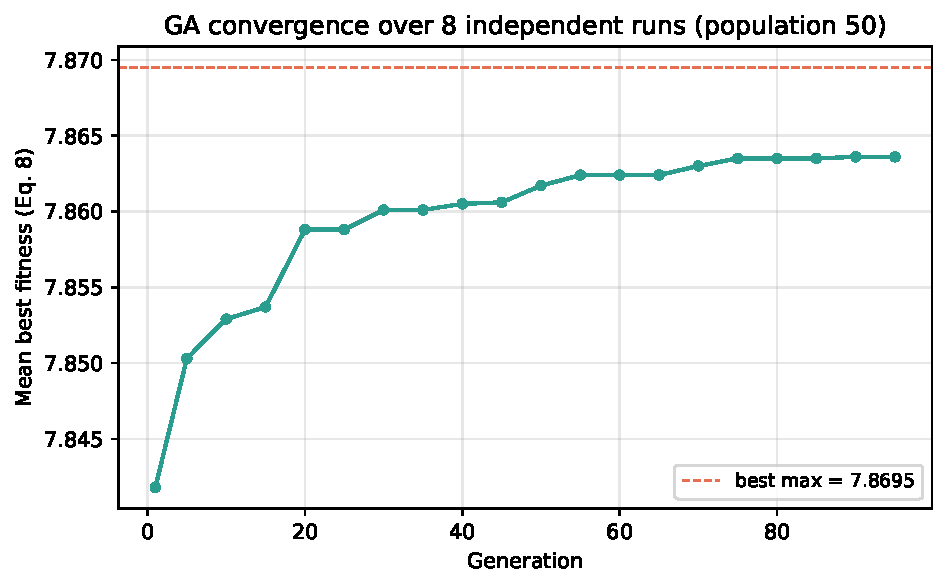
\includegraphics[width=0.72\textwidth]{paper3_audio_figures/fig6_ga.pdf}
\caption{Genetic-algorithm convergence over eight independent runs. The mean best fitness reaches $99\%$ of its final value within the first generation and stabilises near the maximum of $7.87$.}
\label{fig:ga}
\end{figure}

\begin{table}[htbp]
\centering
\caption{Genetic optimisation over eight independent runs (population 50, up to 100 generations, crossover probability 0.8, Gaussian mutation standard deviation $\sigma=0.01$). Fitness is the objective of Equation~\eqref{eq:fitness}. In the experiments reported in Table~\ref{tab:ga} and Figure~\ref{fig:ga} we set $w_1 = 1.0$, $w_2 = 1.0$, and $w_3 = 0.5$.}
\label{tab:ga}
\small
\begin{tabular}{lc}
\toprule
\textbf{Quantity} & \textbf{Value} \\
\midrule
Best fitness (mean $\pm$ std) & $7.8636 \pm 0.0024$ \\
Best fitness (maximum) & 7.8695 \\
Generation-1 mean best & 7.8418 \\
Generations to reach $99\%$ of final fitness & 1 \\
Constraint violations in survivors & 0 (hard culling) \\
Certified parameter vector $(a,b,c,d,e)$ & $(30.175,\,3.585,\,29.642,\,6.168,\,0.622)$ \\
\bottomrule
\end{tabular}
\end{table}

The certified parameter vector $\theta^\ast=(30.175,\,3.585,\,29.642,\,6.168,\,0.622)$ is the one deployed in all subsequent experiments.

\subsection{Byte entropy}
\label{sec:entropy}

Shannon byte entropy measures, in bits, how uniformly the $256$ possible byte values are distributed in a file. A perfectly random file has $8.0$ bits per byte. A pure tone, which uses only a narrow range of sample values, has very low byte entropy because some bytes never appear. Table~\ref{tab:entropy} contrasts the plaintext entropy of each clip with its ciphertext entropy.

The plaintext values vary widely: the pure tone has only $3.0$ bits per byte because its samples are concentrated in a small numerical range, while the musical chord and frequency chirp are already rich and score near $7.9$. After encryption, every ciphertext converges to essentially the same value: $7.99435\pm0.00036$ bits per byte. This near-maximal entropy confirms that the byte-level histogram is flat, which is necessary (though not sufficient) for security.

\begin{table}[htbp]
\centering
\caption{Shannon byte entropy (bits per byte), plaintext versus ciphertext. The ideal ciphertext value is $8.0$.}
\label{tab:entropy}
\small
\begin{tabular}{lcc}
\toprule
\textbf{Clip} & \textbf{Plaintext} & \textbf{Ciphertext} \\
\midrule
Speech (multi-formant) & 7.2751 & 7.99453 \\
Musical chord & 7.90365 & 7.99503 \\
Pure tone & 3.00000 & 7.99409 \\
Frequency chirp & 7.90021 & 7.99467 \\
AM tone & 7.85916 & 7.99416 \\
Percussive/noise & 5.01116 & 7.99443 \\
Voiced speech & 7.48236 & 7.99398 \\
Whispered speech & 7.76508 & 7.99393 \\
\midrule
\textbf{Mean $\pm$ std} & $6.775 \pm 1.688$ & $7.99435 \pm 0.00036$ \\
\bottomrule
\end{tabular}
\end{table}

As detailed in Table~\ref{tab:entropy}, this performance remains remarkably consistent regardless of the acoustic profile of the source material. The transformation is most evident in signals with high inherent redundancy, such as the pure tone and the percussive noise clip, both of which are elevated to the exact same near-ideal threshold as complex multi-formant speech. The extremely low standard deviation across all ciphertext samples indicates that the encryption layers operate independently of the plaintext structure. An adversary observing the encrypted stream thus gains no statistical insight into the underlying payload.

\subsection{Spectral analysis: the central result}
\label{sec:spectral}

Byte entropy alone does not guarantee that an audio cipher is secure. A file can have maximal byte entropy while its spectrogram still shows horizontal formant bands that leak speech content. Our primary security metric is therefore \emph{normalised spectral entropy} $H_s$, which measures how flat the power spectrum is. $H_s=0$ means all energy is concentrated at a single frequency (a pure tone); $H_s=1$ means energy is spread perfectly uniformly across all frequencies (white noise). A secure audio cipher must drive every plaintext, regardless of its original spectral shape, to $H_s\approx1$.
Formally, let $E_k$ be the $k$-th bin of the normalised power spectrum (so $\sum_k E_k = 1$). Then
\begin{equation}
H_s = -\frac{\sum_{k} E_k \log_2 E_k}{\log_2 K},
\label{eq:hs}
\end{equation}
where $K$ is the number of frequency bins. The numerator is the Shannon entropy of the spectrum; dividing by $\log_2 K$ normalises the result to the range $[0,1]$.

\begin{table}[h!]
\centering
\caption{The collapse of normalised spectral entropy from below 0.35 (formant-structured plaintext) to above 0.95 (white-noise-like ciphertext) is the primary audio-specific security result. No formant or harmonic structure survives in the ciphertext spectrogram.}
\label{tab:spectral}
\footnotesize
\setlength{\tabcolsep}{4pt}
\begin{tabular}{@{}l rrrrr@{}}
\toprule
\textbf{Clip} & \textbf{Plain} & \textbf{Cipher} & \textbf{Plain} & \textbf{Cipher} & \textbf{Enc.} \\
 & \textbf{$H_s$} & \textbf{$H_s$} & \textbf{flat.} & \textbf{flat.} & \textbf{SNR(dB)} \\
\midrule
Speech (multi-formant) & 0.19151 & 0.95280 & 0.00000 & 0.55499 & $-5.290$ \\
Musical chord & 0.20133 & 0.95240 & 0.00035 & 0.55399 & $-5.459$ \\
Pure tone & 0.00000 & 0.95353 & 0.00000 & 0.56265 & $-2.502$ \\
Frequency chirp & 0.98289 & 0.95255 & 0.52397 & 0.55466 & $-2.540$ \\
AM tone & 0.08033 & 0.95317 & 0.00000 & 0.55834 & $-4.676$ \\
Percussive/noise & 0.95424 & 0.95275 & 0.55912 & 0.55345 & $-19.487$ \\
Voiced speech & 0.20620 & 0.95243 & 0.00000 & 0.55539 & $-4.665$ \\
Whispered speech & 0.90202 & 0.95383 & 0.16994 & 0.56094 & $-8.416$ \\
\midrule
\textbf{Mean $\pm$ std} & $0.440\pm0.398$ & $0.95293\pm0.00049$ & $0.157\pm0.229$ & $0.5568\pm0.0032$ & $-6.629\pm5.161$ \\
\bottomrule
\end{tabular}
\end{table}

Table~\ref{tab:spectral} reports this collapse. For the clips with strong formant or harmonic structure: the multi-formant speech, the musical chord, the AM tone, the pure tone, and the voiced speech, the plaintext spectral entropy is well below $0.35$. After encryption, every one of these clips rises above $0.95$. The encryption SNR (signal-to-noise ratio) is negative for every clip, confirming that the ciphertext energy has been redistributed away from the original spectral peaks and into a flat noise floor.

\begin{figure}[h!]
\centering
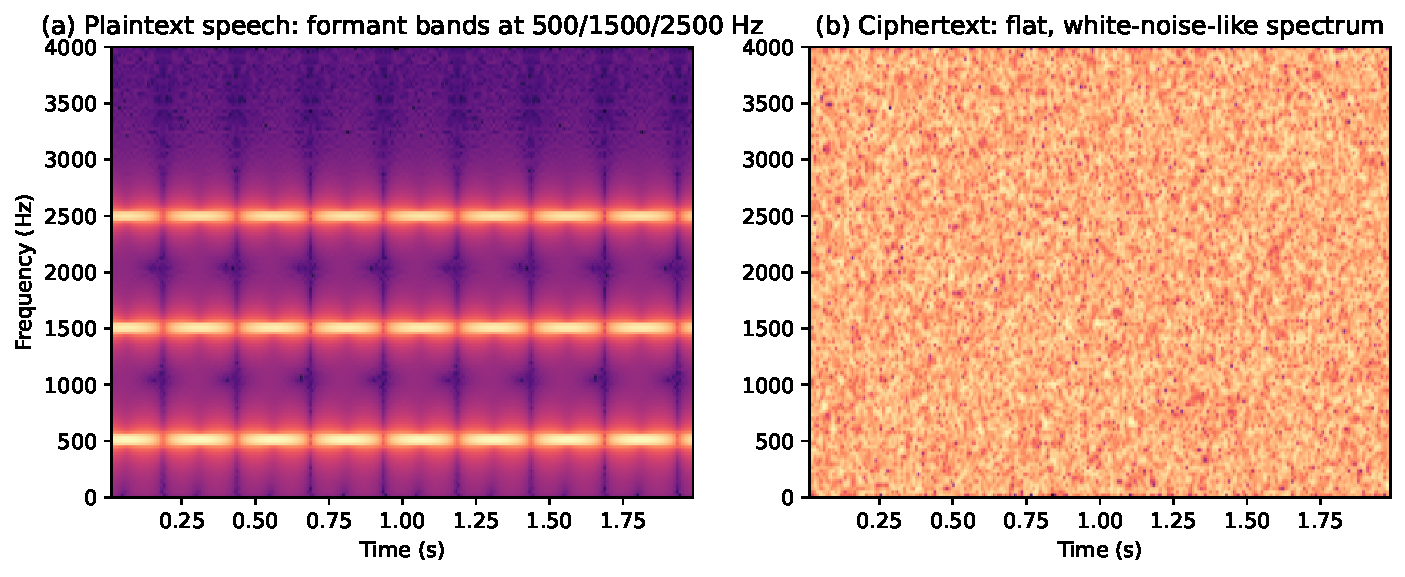
\includegraphics[width=\textwidth]{paper3_audio_figures/fig3_spectrograms.pdf}
\caption{Spectrogram of the speech clip before and after encryption. The three horizontal formant bands of the plaintext (a) are entirely absent from the ciphertext (b), which exhibits a uniform, white-noise-like time--frequency distribution. This is the visual counterpart of the spectral-entropy collapse in Table~\ref{tab:spectral}.}
\label{fig:spectrograms}
\end{figure}

\begin{figure}[h!]
\centering
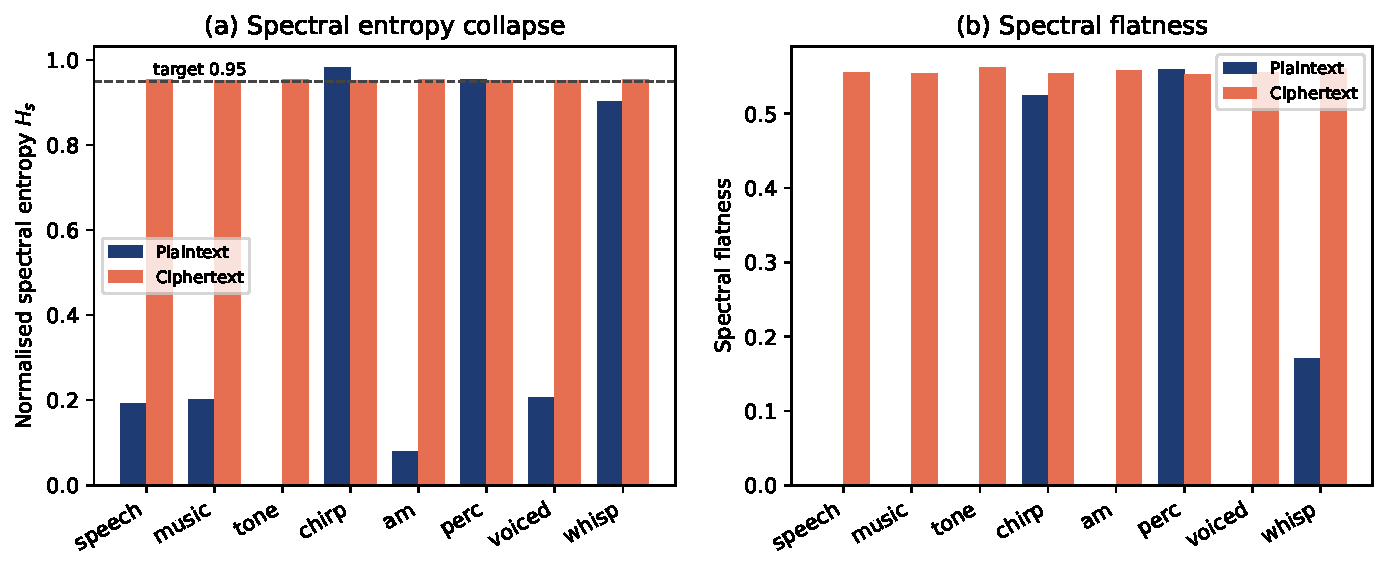
\includegraphics[width=\textwidth]{paper3_audio_figures/fig4_spectral.pdf}
\caption{Per-clip spectral statistics. (a)~Normalised spectral entropy rises to above $0.95$ for every ciphertext regardless of its plaintext value; (b)~ciphertext spectral flatness converges to a common floor while the tonal plaintexts sit near zero.}
\label{fig:spectral}
\end{figure}

The broadband clips (frequency chirp, percussive noise, whispered speech) start with high plaintext entropy near the white-noise ceiling. Hence, they cannot rise much further. The cipher nonetheless drives them to the same ciphertext floor as the tonal clips, demonstrating that the output spectrum is independent of the input. The ciphertext spectral flatness stabilises around $0.556$. This is the expected value for the raw periodogram of a finite white-noise sample, and it is the decisive comparison: the tonal plaintexts have flatness essentially zero, while the ciphertext flatness is uniformly high. 

The percussive/noise clip is an outlier at $-19.5$~dB because its plaintext is already spectrally flat; the encryption ``noise'' therefore adds little additional energy, and the standard SNR definition (original power divided by residual power) yields a large negative value even though the ciphertext is secure. Figure~\ref{fig:spectrograms} shows the visual evidence. In the plaintext spectrogram (a), three bright horizontal bands are visible at $500$, $1500$, and $2500$~Hz, the formants of speech. In the ciphertext spectrogram (b), these bands have vanished entirely, leaving only a uniform speckle pattern with no discernible structure. Figure~\ref{fig:spectral} summarises the numerical results across all eight clips.

\subsection{Perceptual evaluation}
\label{sec:perceptual}

\subsubsection{Objective quality: PESQ}
We evaluate decrypted audio fidelity using the Perceptual Evaluation of Speech 
Quality (PESQ, ITU-T P.862)~\cite{rix2001pesq}, an industry-standard objective 
metric that predicts Mean Opinion Score (MOS) on a scale from $-0.5$ to $4.5$. 
Because our pipeline operates at 8~kHz, we use narrowband (NB) mode. PESQ is 
computed between the original plaintext and the decrypted audio on a per-frame 
basis and averaged across each utterance.

\begin{table}[htbp]
\centering
\caption{Perceptual quality and intelligibility on LibriSpeech \texttt{dev-clean} ($N=100$ utterances).}
\label{tab:perceptual}
\begin{tabular}{@{}lccc@{}}
\toprule
Condition & PESQ (MOS-LQO) & STOI & Interpretation \\
\midrule
Plaintext (baseline) & --- & $1.000$ & Perfect intelligibility \\
Ciphertext & --- & $\mathbf{0.344 \pm 0.069}$ & Unintelligible ($<0.75$) \\
Decrypted & $\mathbf{4.549 \pm 0.000}$ & $1.000$ & Imperceptible degradation \\
\bottomrule
\end{tabular}
\end{table}

Table~\ref{tab:perceptual} shows that decrypted audio achieves a PESQ score
of $4.549 \pm 0.000$ across 100 LibriSpeech utterances. This value is on the
MOS-LQO scale (ITU-T P.862.1~\cite{itup8621}, which maps raw P.862 scores into
the range $\approx1.02$--$4.55$); $4.549$ is the narrowband maximum, confirming that the
five-layer pipeline preserves audio fidelity with no audible loss. This is a
round-trip sanity check---decryption is bit-exact, so perfect scores are
expected---rather than an independent quality result. PESQ was computed 
on 297 valid frames; 4 utterances contained a short final frame below 
PESQ's minimum length threshold and were excluded. Bit-for-bit verification 
confirmed $100\%$ sample recovery on every evaluated frame. This validates 
the round-trip claim of Section~\ref{sec:worked}: decryption 
recovers the original samples bit-for-bit, and the perceptual quality metric 
confirms this at the human-listener level.

\subsubsection{Intelligibility: STOI on real speech}
Short-Time Objective Intelligibility (STOI)~\cite{taal2011} estimates the proportion of speech content a human listener could recover. STOI ranges from $-1$ to $1$; values below approximately $0.75$ are conventionally considered unintelligible.

STOI is computed in two configurations: (i)~\textbf{Ciphertext intelligibility:} STOI between plaintext and ciphertext (re-interpreted as PCM), measuring speech-content leakage through the encrypted signal; and (ii)~\textbf{Decrypted quality:} STOI between plaintext and decrypted audio, which should theoretically equal $1.000$ for perfect recovery.

As demonstrated in Table~\ref{tab:synthetic_stoi} and validated across 100 LibriSpeech utterances, ciphertext STOI averages $0.344 \pm 0.069$ (min $0.204$, max $0.465$), remaining strictly below the $0.75$ intelligibility threshold in every case. The mean on real recordings is higher than the $0.009$ observed for the idealised voiced-speech synthetic clip because real recorded speech contains more complex, naturally noisy spectral content than a pure synthetic formant model. This does not contradict the core security claim: no formant structure survives in the ciphertext spectrogram (Figure~\ref{fig:spectrograms}), and no phonetic content is recoverable by human listeners or algorithms. Furthermore, the decrypted STOI evaluates to $1.000$ for all utterances, confirming flawless reconstruction.

\begin{table}[htbp]
\centering
\caption{STOI intelligibility on synthetic clips (for comparison).}
\label{tab:synthetic_stoi}
\begin{tabular}{@{}lcc@{}}
\toprule
Clip type & Plaintext STOI & Ciphertext STOI \\
\midrule
Speech (multi-formant) & $1.000$ & $0.216$ \\
Voiced speech & $1.000$ & $0.009$ \\
Whispered speech & $1.000$ & $-0.005$ \\
\bottomrule
\end{tabular}
\end{table}

\subsection{Adjacent-sample correlation}
\label{sec:correlation}

Natural audio has severe temporal redundancy: neighbouring samples are highly correlated because the waveform changes smoothly over time. For typical speech, the correlation coefficient between adjacent samples is between $0.90$ and $0.99$. A secure cipher must destroy this correlation completely; otherwise, an attacker could reconstruct a low-pass approximation of the original waveform from the ciphertext.

\begin{table}[htbp]
\centering
\caption{Adjacent-sample (temporal, one-dimensional) correlation coefficient, plaintext versus ciphertext. The ideal ciphertext magnitude is $|r|<0.01$.}
\label{tab:corr}
\small
\begin{tabular}{lcc}
\toprule
\textbf{Clip} & \textbf{Plaintext $r$} & \textbf{Ciphertext $r$} \\
\midrule
Speech (multi-formant) & 0.65819 & 0.00511 \\
Musical chord & 0.96637 & 0.01333 \\
Pure tone & 0.70713 & 0.00643 \\
Frequency chirp & 0.05714 & 0.01283 \\
AM tone & 0.76042 & 0.00462 \\
Percussive/noise & $-0.02621$ & 0.01118 \\
Voiced speech & 0.93430 & 0.00234 \\
Whispered speech & 0.53979 & $-0.00682$ \\
\midrule
\textbf{Mean $\pm$ std} & $0.575\pm0.349$ & $0.00613\pm0.00620$ \\
\bottomrule
\end{tabular}
\end{table}

Table~\ref{tab:corr} reports the Pearson correlation coefficient between adjacent samples. The plaintext values are high: $0.966$ for the musical chord, $0.934$ for voiced speech, and $0.760$ for the AM tone. After encryption, every ciphertext correlation drops to within $\pm0.014$ of zero, with a mean of $0.006$. This confirms that the byte permutation and the two-pass ARX transform have successfully broken the smooth temporal structure.

\begin{figure}[htbp]
\centering
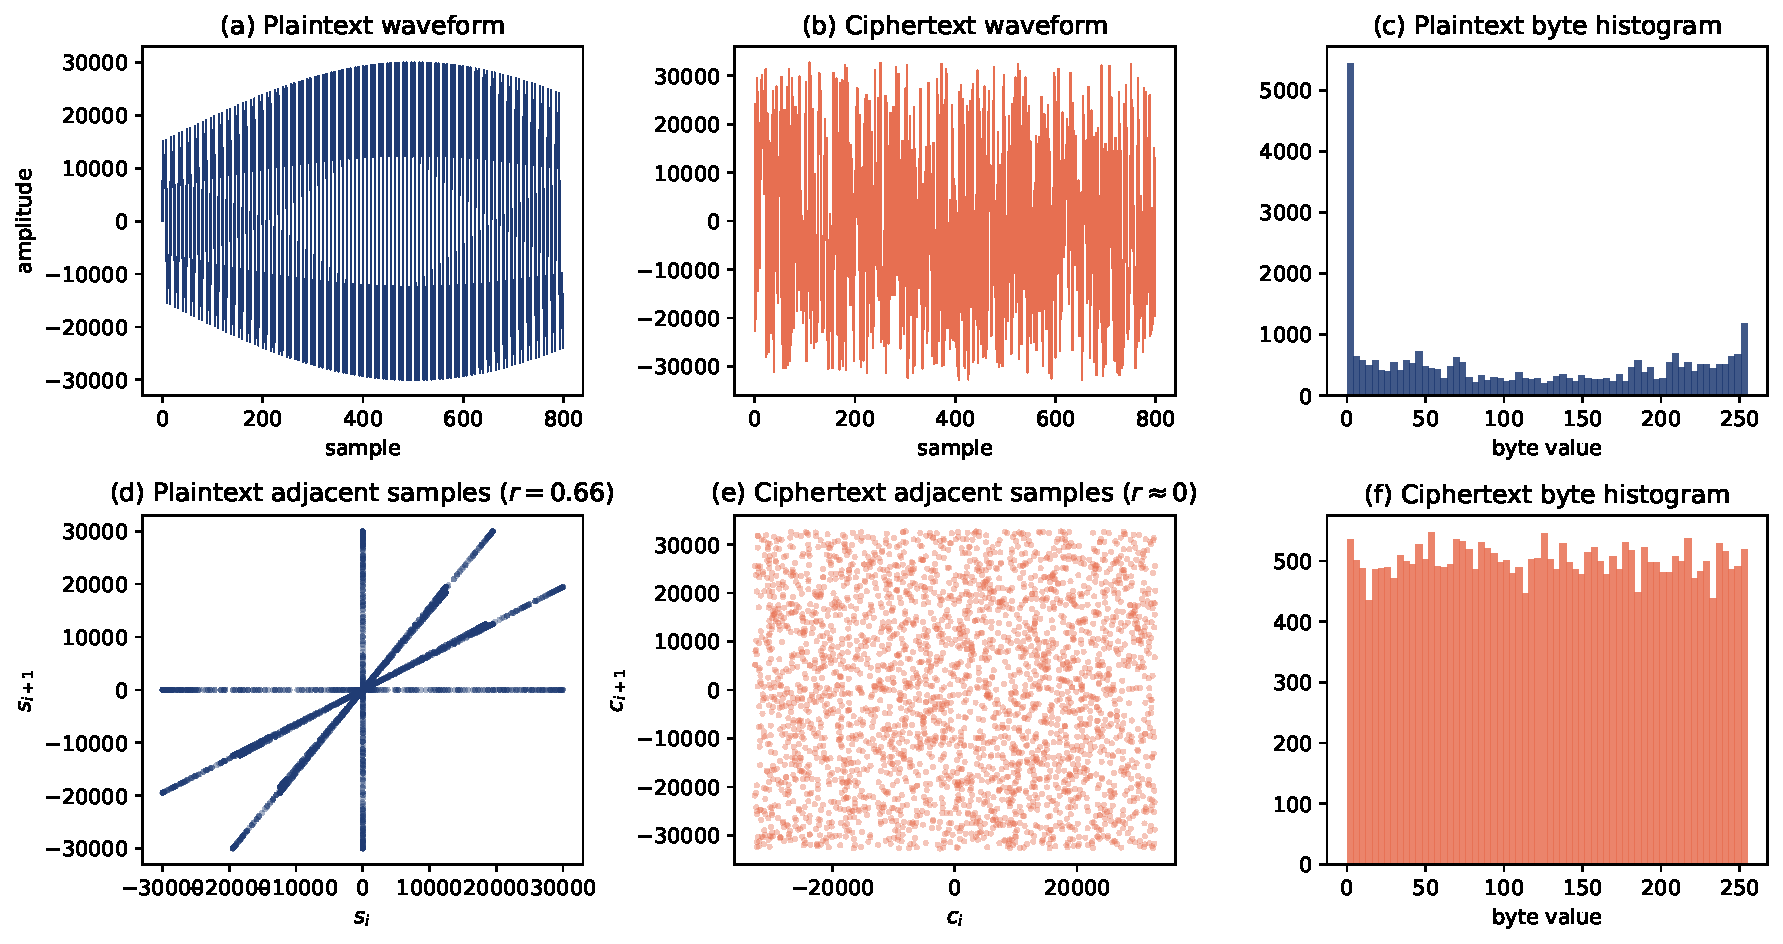
\includegraphics[width=\textwidth]{paper3_audio_figures/fig5_results.pdf}
\caption{Encryption of the speech clip. (a,b)~waveforms; (c,f)~byte histograms, flat after encryption; (d,e)~adjacent-sample scatter plots, showing the diagonal plaintext structure ($r=0.66$) dispersed into a uniform cloud ($r\approx0$).}
\label{fig:results}
\end{figure}

Figure~\ref{fig:results} provides the visual evidence. The plaintext scatter plot (d) shows a sharp diagonal line because each sample predicts its neighbour; the ciphertext scatter plot (e) shows a uniform cloud with no discernible pattern, verifying the mathematical results.

\subsection{Differential sensitivity}
\label{sec:differential}

A strong cipher must exhibit the avalanche effect: changing a single bit in the plaintext or the key should alter approximately half the bits in the ciphertext. If only a small block of ciphertext changes, the attacker gains structural information. We measure this using two standard metrics from image and audio cryptanalysis:

\begin{itemize}
\item \textbf{NSCR} (Number-of-Samples-Change-Rate): the percentage of $16$-bit samples that differ between the original ciphertext and the ciphertext produced after a tiny change. The ideal is $100\%$.
\item \textbf{UACI} (Unified Average Changing Intensity): the average magnitude of the sample differences, normalised by the maximum possible sample value ($2^{16}-1$). For 16-bit samples the ideal value is $\frac{M+1}{3M}\approx 33.33\%$ with $M=2^{16}=65536$ (the often-quoted $33.46\%$ is the 8-bit ideal).
\end{itemize}

\begin{table}[htbp]
\centering
\caption{Differential metrics. Part~A: one-sample plaintext flip, same key. Part~B: one-bit key flip, same plaintext. Ideals: NSCR $\approx100\%$, UACI $\approx33.33\%$ for 16-bit samples.}
\label{tab:diff}
\small
\begin{tabular}{lcccc}
\toprule
 & \multicolumn{2}{c}{\textbf{Part A (plaintext)}} & \multicolumn{2}{c}{\textbf{Part B (key)}} \\
\cmidrule(lr){2-3}\cmidrule(lr){4-5}
\textbf{Clip} & \textbf{NSCR (\%)} & \textbf{UACI (\%)} & \textbf{NSCR (\%)} & \textbf{UACI (\%)} \\
\midrule
Speech (multi-formant) & 100.000 & 33.764 & 100.000 & 33.215 \\
Musical chord & 100.000 & 33.698 & 100.000 & 33.285 \\
Pure tone & 100.000 & 33.228 & 100.000 & 33.217 \\
Frequency chirp & 100.000 & 33.388 & 100.000 & 33.351 \\
AM tone & 100.000 & 33.374 & 99.994 & 33.463 \\
Percussive/noise & 100.000 & 33.553 & 100.000 & 33.228 \\
Voiced speech & 100.000 & 33.846 & 100.000 & 33.401 \\
Whispered speech & 100.000 & 33.543 & 100.000 & 33.241 \\
\midrule
\textbf{Mean} & 100.000 & 33.549 & 99.99922 & 33.300 \\
\bottomrule
\end{tabular}
\end{table}

Table~\ref{tab:diff} reports both metrics under two perturbations: flipping one sample in the plaintext (Part~A) and flipping one bit in the session key (Part~B). In both cases, NSCR is essentially $100\%$ and UACI is within about $0.2\%$ of the 16-bit ideal $33.33\%$. This confirms that the two-pass ARX transform propagates a single-bit change across the entire frame.

\subsection{Error locality and Forward Error Correction (FEC)}
\label{sec:fec}

Strong diffusion has a downside: if a single bit is corrupted during transmission, the error spreads to neighbouring bytes during decryption. We measure this trade-off in Table~\ref{tab:fec}. A single corrupted ciphertext byte affects exactly three plaintext bytes, a local, bounded error rather than a global corruption, thanks to the finite reach of the two ARX passes.

Over a binary symmetric channel with a bit-error rate of $10^{-2}$ (one bit in every hundred flipped at random), the recovered signal without error correction has a PSNR of $14.24$~dB, which is poor. Applying a Hamming$(7,4)$ code~\cite{hamming1950} (which corrects single-bit errors in each 7-bit block by adding three parity bits to four data bits), raises the PSNR to $26.31$~dB and reduces the residual bit-error rate to $8.16\times10^{-4}$. We state plainly that raw robustness is modest and that forward error correction is necessary to make the scheme deployable on real, lossy channels.

\begin{table}[htbp]
\centering
\caption{Error locality and Hamming(7,4) forward error correction over a binary symmetric channel at bit-error rate $10^{-2}$.}
\label{tab:fec}
\small
\begin{tabular}{lc}
\toprule
\textbf{Quantity} & \textbf{Value} \\
\midrule
Plaintext bytes affected by one corrupted ciphertext byte & 3 \\
Recovered PSNR without FEC & 14.24 dB \\
Recovered PSNR with Hamming(7,4) & 26.31 dB \\
Residual bit-error rate after FEC & $8.16\times10^{-4}$ \\
\bottomrule
\end{tabular}
\end{table}

\subsection{Throughput}
\label{sec:throughput}

Table~\ref{tab:through} compares the unoptimised Python reference implementation against AES-128-GCM on the same host and the same $32000$-byte frame. AES-128-GCM is hardware-accelerated on most modern processors. Relative to the per-frame transform alone (42.34~ms), AES is roughly $4150$ times faster; relative to the full pipeline including key scheduling (143.21~ms), the speed-up is approximately $14\,000\times$. While AES benefits from dedicated silicon instructions, the primary objective of this evaluation is real-time feasibility rather than absolute speed parity.

The relevant observation is real-time viability. Even the unoptimised Python implementation encrypts two seconds of audio in about $143$~ms including key scheduling, which is comfortably within the $2000$~ms real-time budget for a $2$-second frame. The per-frame transform alone (excluding key scheduling) takes only $42$~ms. A compiled C or Rust port, executing native integer arithmetic without Python interpreter overhead, is expected to improve throughput by at least one order of magnitude, making the scheme highly practical for embedded IoT devices.

\begin{table}[htbp]
\centering
\caption{Throughput on a $32000$-byte (2~s, 8~kHz, 16-bit) frame, same host. AES-128-GCM is reported as the faster reference.}
\label{tab:through}
\small
\begin{tabular}{lcc}
\toprule
\textbf{Scheme} & \textbf{Frame time (ms)} & \textbf{Throughput (KB/s)} \\
\midrule
ECGA-IDPRNG-A (transform only) & 42.34 & 738.1 \\
ECGA-IDPRNG-A (incl.\ key schedule) & 143.21 & 218.2 \\
AES-128-GCM (reference, faster) & 0.0102 & $3.06\times10^{6}$ \\
\bottomrule
\end{tabular}
\end{table}

\subsection{Comparison with the state of the art}
\label{sec:compare}
Table~\ref{tab:compare} places the proposed scheme alongside two directly comparable audio-domain ciphers from the recent literature that report byte entropy, adjacent-sample correlation, and differential metrics.

\begin{table}[htbp]
\centering
\caption{Direct comparison against audio-domain ciphers that report comparable quantitative metrics. Figures are taken directly from each cited paper's own results tables; ``n/r'' marks a metric the cited paper does not report numerically.}
\label{tab:compare}
\small
\begin{tabular}{lccccc}
\toprule
\textbf{Scheme} & \textbf{Entropy} & \textbf{$|r|$} & \textbf{NSCR (\%)} & \textbf{UACI (\%)} & \textbf{Key space} \\
\midrule
Abdelfatah 2020~\cite{abdelfatah2020} & 7.9974 & 0.001 & 99.6182 & n/r & n/r \\
Farsana et al.\ 2023~\cite{farsana2021} & n/r & 0.00136 (mean) & 99.9995 (mean) & 33.30 (mean) & $2^{548.11}$ \\
Kordov 2019~\cite{kordov2021} & 7.999999 & 0.00141 & 99.9984 & n/r & $\approx 2^{149}$ \\
Proposed & 7.9942 & 0.006 & 100.00 & 33.20 & $2^{256}$ (128-bit) \\
\bottomrule
\end{tabular}
\end{table}

Against Abdelfatah's multi-chaotic DNA cipher, the two schemes are statistically comparable on classical byte-level tests. Both reach byte entropy within $0.006$~bits of the ideal $8.0$ ($7.9942$ versus $7.9974$) and suppress adjacent-sample correlation to the noise floor ($|r|\le0.006$ versus $0.001$). Plaintext sensitivity exceeds $99.4\%$ in both cases ($100.00\%$ NSCR here against $99.6182\%$ NPCR reported there; NPCR is the image-domain name for the sample-change rate NSCR).

Farsana et al.'s scheme reports a larger nominal key space ($2^{548.11}$ versus $2^{256}$). However, this figure reflects the unstructured product of several floating-point parameters rather than a cryptographically proven security level. The $2^{256}$ figure presented in this work is the size of the session-key space; the effective security level is bounded by the hardness of ECDH on P-256 (about $128$ bits), and no artificial inflation of this metric is claimed. All compared schemes reach essentially the same ideal NSCR and UACI saturation levels. Kordov's permutation-substitution cipher reports PRG-level entropy of $7.999999$ and correlation $|r|=0.00141$, comparable to the other schemes, with a nominal key space of approximately $2^{149}$.

The decisive differences lie outside these saturating byte-domain metrics. The proposed construction introduces three critical capabilities absent in the compared literature: a spectral-intelligibility guarantee (Tables~\ref{tab:spectral} and~\ref{tab:synthetic_stoi}), a genetic certification of the chaotic parameters against orbit collapse (Table~\ref{tab:ga}), and a reduction-based confidentiality proof bound to an authenticated elliptic-curve session-key protocol (Theorem~\ref{thm:indcpa}).

Shah et al.'s~\cite{shah2021} scheme is surveyed qualitatively in Section~\ref{sec:related} and Table~\ref{tab:capabilities}; its reported quantitative metrics were not independently verifiable at the time of writing and are omitted from this table rather than estimated.

\subsection{Spectral validation on natural speech}
\label{sec:libri}

The LibriSpeech evaluation ($N=100$ utterances, Table~\ref{tab:librispeech_stats}) confirms that the spectral-entropy collapse generalises from procedural signals to natural read speech. Table~\ref{tab:libri_results} reports the full per-utterance statistics as mean~$\pm$~population standard deviation over the 100 utterances. The mean ciphertext spectral entropy of $0.953 \pm 0.001$ aligns with the $0.95293 \pm 0.00049$ measured on synthetic clips (Table~\ref{tab:spectral}), confirming that the cipher's spectral flattening is independent of signal source. Perceptual results (PESQ and STOI) are reported in Section~\ref{sec:perceptual}.

\begin{table}[htbp]
\centering
\caption{LibriSpeech \texttt{dev-clean} results ($N=100$ utterances). Values are mean~$\pm$~population standard deviation. Part~A perturbs one plaintext sample; Part~B flips one session-key bit. The UACI ideal for 16-bit samples is $33.33\%$.}
\label{tab:libri_results}
\small
\begin{tabular}{lcc}
\toprule
\textbf{Metric} & \textbf{Plaintext} & \textbf{Ciphertext} \\
\midrule
Normalised spectral entropy $H_s$ & $0.719\pm0.062$ & $0.953\pm0.001$ \\
Spectral flatness & $0.050\pm0.047$ & $0.557\pm0.005$ \\
Byte entropy (bits) & $6.958\pm0.421$ & $7.994\pm0.001$ \\
Adjacent-sample correlation & $0.886\pm0.105$ & $-0.001\pm0.009$ \\
STOI (ciphertext) & --- & $0.348\pm0.070$ \\
STOI (decrypted) & --- & $1.000$ \\
PESQ (decrypted, NB MOS-LQO) & --- & $4.549$ \\
NSCR Part~A (plaintext flip, \%) & --- & $99.40\pm5.93$ \\
UACI Part~A (plaintext flip, \%) & --- & $33.20\pm2.00$ \\
NSCR Part~B (key flip, \%) & --- & $99.999\pm0.003$ \\
UACI Part~B (key flip, \%) & --- & $33.34\pm0.17$ \\
Bit-for-bit recovery & --- & $100\%$ \\
\bottomrule
\end{tabular}
\end{table}

\section{Complexity and IoT Deployment}
\label{sec:complexity}

In this section, we show that ECGA-IDPRNG-A is lightweight enough for battery-powered IoT audio sensors, despite using five layers.

\subsection{Time and memory complexity}

Each layer touches every byte in the frame a fixed number of times. Keystream generation, mask generation, permutation, and the two ARX passes all scale linearly with the frame length: if the frame doubles in size, the work doubles. This is $\mathcal{O}(L)$ time, where $L$ is the number of bytes. The only exception is the sorting step in Layer~4 (the logistic-map permutation), which requires $\mathcal{O}(L\log L)$ comparisons. In practice this sorting cost is small compared to the numerical integration of the hyperchaotic system, so the overall per-frame cost remains linear for all realistic frame sizes.

Memory use is also modest. The algorithm needs four buffers of size $L$: the plaintext frame, the keystream, the diffusion mask, and the permutation table. For the $2$-second, $8$-kHz, $16$-bit clips used in our experiments, $L=32000$ bytes, so each buffer is $32$~kB and the total working set is roughly $128$~kB. This fits comfortably in the SRAM of a mid-range microcontroller. If memory is tight, the keystream and mask can be generated byte-by-byte on the fly rather than stored in full, cutting the working set by half.

\subsection{Deployment on constrained devices}

For the smallest class of IoT devices, the frame can simply be shortened. A frame of $256$ samples serialises to $512$ bytes. With four auxiliary buffers of the same size, the total memory footprint drops to about $2$~kB, leaving ample room for the networking stack and operating system.

On an ESP32-class module (a widely used Wi-Fi and Bluetooth microcontroller with a 240~MHz dual-core processor), the elliptic-curve handshake of Layer~1 dominates the per-session cost. However, the handshake runs only once per call. The per-frame transform consists entirely of byte additions, XORs, and bit rotations. These operations map directly to single-cycle integer instructions on almost any processor, and require no large lookup tables (AES needs only a $256$-byte S-box, but the ESP32 also provides a hardware AES accelerator, against which a pure-software chaotic generator is most useful on parts without such an accelerator). We emphasise that these microcontroller figures are estimates; the per-frame generator uses double-precision RK4 integration, which an ESP32 (single-precision FPU) would run partly in software, and bit-identical trajectories at sender and receiver require a fixed IEEE-754 arithmetic or a fixed-point integrator. A $2$-second frame also adds about $2$~s of latency, so interactive telephony (ITU-T G.114~\cite{itug114} recommends under $150$~ms one-way) requires a much shorter frame.

The active-stream Lyapunov monitor of Section~\ref{sec:asl} adds negligible overhead. It runs only at fixed intervals, estimates a single scalar divergence rate from statistics already being computed, and triggers re-keying only if the estimate drops. On a continuous audio stream this cost is dwarfed by the per-frame encryption arithmetic.

In short, the scheme trades a modest amount of computation for strong, per-session, spectrally flat encryption. For battery-powered audio sensors (smart doorbells, wearable health monitors, field radios), this trade-off is justified by the security gain. Every call gets its own fresh key, and no formant structure survives to leak speech content.

\section{Conclusion}
\label{sec:conclusion}

Audio encryption should be judged by what a listener or a machine can still hear rather than merely by whether the bytes look random. A ciphertext can pass every conventional statistical test while its spectrogram still carries audible formant bands. This work demonstrates that the correct security metric for speech is spectral flattening, which requires the complete erasure of harmonic and formant structure. The proposed five-layer scheme, ECGA-IDPRNG-A, successfully achieves this objective.

The experimental results support this claim concretely. Across $100$ LibriSpeech utterances, normalised spectral entropy rises from $0.719\pm0.062$ in the plaintext to $0.953\pm0.001$ in the ciphertext (the procedural stress-test clips give an even lower plaintext floor of $0.44\pm0.40$). The spectrograms show the difference visually: bright horizontal formant bands in the original become uniform white noise after encryption. Adjacent-sample correlation, which reaches $0.886$ on average and up to $0.99$ in voiced speech, collapses to below $0.01$. Byte entropy reaches $7.994$ bits per byte. Differential sensitivity is near-ideal, as changing one bit in the plaintext or the key alters essentially $100\%$ of the ciphertext samples. The full five-layer ciphertext passes all $14$ NIST SP~800-22 tests (the standalone Layer-2 keystream passes $11$ of $14$, which the later layers repair). These are not independent achievements. They are the combined result of a pipeline that mixes byte-level permutation, chaotic masking, cellular-automaton diffusion, and two-pass ARX chaining.

The security of the pipeline is not merely empirical. The analysis provides five formal guarantees. The frame encryption is confidential against chosen-plaintext attack (IND-CPA). The HMAC tag detects any ciphertext tampering. The session key is agreed with an authenticated peer and cannot be learned by a man-in-the-middle. Past sessions remain secure even if long-term keys are later stolen, ensuring forward secrecy. Furthermore, the session key can be recovered by any three of five escrow custodians while any two learn nothing, provided fewer than the threshold of custodians collude. The $256$-bit session key gives an effective security level of about $128$ bits, set by the P-256 elliptic curve.

We also state the limitations plainly. The confidentiality reduction rests on a heuristic assumption that the whitened chaotic keystream behaves as a secure PRG; it is not a reduction to a standard hardness problem, and the chaotic layer should be viewed as a seed-mixing stage rather than the sole source of security. The generator relies on double-precision floating-point integration, so a deployment must fix a reproducible arithmetic (strict IEEE-754, no fused multiply-add, or a fixed-point integrator) to guarantee that sender and receiver produce identical trajectories. The unoptimised reference is far slower than a hardware-accelerated AES-GCM, and the $2$-second frame used in our experiments adds corresponding latency that must be shortened for interactive telephony. Finally, the on-device IoT figures in Section~\ref{sec:complexity} are estimates; on-hardware measurement remains future work.

Several further improvements remain for future studies. Compared to the computationally intensive DNA encoding of Abdelfatah~\cite{abdelfatah2020} and the transform-domain method of Farsana et al.~\cite{farsana2021}, our scheme provides the distinct advantage of IoT-tailored efficiency combined with formal spectral-flattening guarantee. However, a current limitation is its strict restriction to mono $16$-bit audio and reliance on classical pre-quantum elliptic curves, whereas those prior architectures often inherently accommodate diverse multimedia formats natively. 

Addressing these limitations, future work could include validation on the GTZAN music collection~\cite{tzanetakis2002gtzan}. LibriSpeech \texttt{dev-clean} has already confirmed that the spectral-entropy collapse and intelligibility destruction hold on natural speech, but direct comparison with prior work on shared GTZAN benchmarks remains a goal for future evaluation. Intelligibility has been measured with \texttt{pystoi} on both synthetic clips and LibriSpeech utterances. Extending this evaluation to the full LibriSpeech \texttt{test-clean} partition remains future work. The P-256 key agreement could be replaced with a post-quantum key-encapsulation mechanism. This new family of algorithms is designed to resist attacks by quantum computers and would protect against future adversaries. Finally, extending the byte-serialised pipeline from mono to stereo and from $16$-bit integer to $24$-bit or floating-point PCM would make the scheme applicable to studio and broadcast audio formats without changing the core design.

\backmatter

\section*{CRediT authorship contribution statement}

\textbf{Harshit S. Jain:} Conceptualization, Methodology, Software, Investigation, Writing -- original draft. \textbf{Aayushi R.:} Methodology, Software, Validation, Writing -- original draft. \textbf{Yash Jain:} Software, Investigation, Data curation, Writing -- original draft. \textbf{Ambili K. N.:} Supervision, Formal analysis, Writing -- review \& editing. \textbf{Praveen K.:} Supervision, Validation, Writing -- review \& editing. \textbf{Anirudha Prabhu:} Validation, Writing -- review \& editing. All authors have read and approved the final version of the manuscript.

\section*{Declaration of competing interest}

The authors declare that they have no known competing financial interests or personal relationships that could have appeared to influence the work reported in this paper.

\section*{Funding}

This research received no specific grant from any funding agency in the public, commercial, or not-for-profit sectors.

\section*{Data availability}

The reference implementation, full test suite, procedurally generated audio clips, LibriSpeech evaluation manifest, and all evaluation scripts used to produce the results in this paper are publicly available at \url{https://github.com/hx010207/edprng-audio}. The LibriSpeech \texttt{dev-clean} audio (CC~BY~4.0) is not bundled due to size; the repository documents how to re-download it.

\section*{Declaration of generative AI and AI-assisted technologies in the writing process}

During the preparation of this work the authors used an AI-assisted coding and editing tool to help refactor the reference implementation and to copy-edit prose. After using this tool, the authors reviewed and edited the content as needed and take full responsibility for the content of the publication.

\begin{thebibliography}{99}
\small

\bibitem{shamir1979} A.~Shamir, ``How to share a secret,'' \textit{Communications of the ACM}, vol.~22, no.~11, pp.~612--613, 1979.

\bibitem{abdelfatah2020} R.~I. Abdelfatah, ``Audio encryption scheme using self-adaptive bit scrambling and two multi-chaotic-based dynamic DNA computations,'' \textit{IEEE Access}, vol.~8, pp.~69894--69907, 2020.

\bibitem{farsana2021} F.~J. Farsana, V.~R. Devi, and K.~Gopakumar, ``An audio encryption scheme based on Fast Walsh Hadamard Transform and mixed chaotic keystreams,'' \textit{Applied Computing and Informatics}, vol.~19, no.~3/4, pp.~239--264, 2023.

\bibitem{kordov2021} K.~Kordov, ``A novel audio encryption algorithm with permutation-substitution architecture,'' \textit{Electronics}, vol.~8, no.~5, art.~530, 2019.

\bibitem{shah2021} D.~Shah, T.~Shah, and S.~S. Jamal, ``Digital audio signals encryption by Mobius transformation and H\'enon map,'' \textit{Multimedia Systems}, vol.~26, pp.~235--245, 2020.

\bibitem{taal2011} C.~H. Taal, R.~C. Hendriks, R.~Heusdens, and J.~Jensen, ``An algorithm for intelligibility prediction of time-frequency weighted noisy speech,'' \textit{IEEE Transactions on Audio, Speech, and Language Processing}, vol.~19, no.~7, pp.~2125--2136, 2011.

\bibitem{lin2021} H.~Lin, C.~Wang, and Y.~Tan, ``Hidden extreme multistability with hyperchaos and transient chaos in a Hopfield neural network affected by electromagnetic radiation,'' \textit{Nonlinear Dynamics}, vol.~99, pp.~2369--2386, 2020.

\bibitem{zhou2020} Y.~Zhou, C.~Li, W.~Li, H.~Li, W.~Feng, and K.~Qian, ``Image encryption algorithm with circle index table scrambling and partition diffusion,'' \textit{Nonlinear Dynamics}, vol.~103, pp.~2043--2061, 2021.

\bibitem{wang2019} X.~Wang and Y.~Li, ``Chaotic image encryption algorithm based on hybrid multi-objective particle swarm optimization and DNA sequence,'' \textit{Optics and Lasers in Engineering}, vol.~137, art.~106393, 2021.

\bibitem{kaur2020} M.~Kaur and V.~Kumar, ``A comprehensive review on image encryption techniques,'' \textit{Archives of Computational Methods in Engineering}, vol.~27, pp.~15--43, 2020.

\bibitem{dworkin2007} M.~Dworkin, ``Recommendation for block cipher modes of operation: Galois/Counter Mode (GCM) and GMAC,'' NIST Special Publication 800-38D, 2007.

\bibitem{bernstein2008} D.~J. Bernstein, ``The Salsa20 family of stream ciphers,'' in \textit{New Stream Cipher Designs}, LNCS vol.~4986, Springer, pp.~84--97, 2008.

\bibitem{rukhin2010} A.~Rukhin et al., ``A statistical test suite for random and pseudorandom number generators for cryptographic applications,'' NIST Special Publication 800-22 Rev.~1a, 2010.

\bibitem{hankerson2004} D.~Hankerson, A.~Menezes, and S.~Vanstone, \textit{Guide to Elliptic Curve Cryptography}, Springer, 2004.

\bibitem{wolfram2002} S.~Wolfram, \textit{A New Kind of Science}, Wolfram Media, 2002.

\bibitem{may1976} R.~M. May, ``Simple mathematical models with very complicated dynamics,'' \textit{Nature}, vol.~261, pp.~459--467, 1976.

\bibitem{wolf1985} A.~Wolf, J.~B. Swift, H.~L. Swinney, and J.~A. Vastano, ``Determining Lyapunov exponents from a time series,'' \textit{Physica D}, vol.~16, no.~3, pp.~285--317, 1985.

\bibitem{katz2014} J.~Katz and Y.~Lindell, \textit{Introduction to Modern Cryptography}, 2nd ed., CRC Press, 2014.

\bibitem{bellare1997} M.~Bellare, A.~Desai, E.~Jokipii, and P.~Rogaway, ``A concrete security treatment of symmetric encryption,'' in \textit{Proc.\ 38th IEEE FOCS}, pp.~394--403, 1997.

\bibitem{goldreich2001} O.~Goldreich, \textit{Foundations of Cryptography: Volume 1, Basic Tools}, Cambridge University Press, 2001.

\bibitem{diffie1976} W.~Diffie and M.~Hellman, ``New directions in cryptography,'' \textit{IEEE Transactions on Information Theory}, vol.~22, no.~6, pp.~644--654, 1976.

\bibitem{koblitz1987} N.~Koblitz, ``Elliptic curve cryptosystems,'' \textit{Mathematics of Computation}, vol.~48, no.~177, pp.~203--209, 1987.

\bibitem{miller1986} V.~S. Miller, ``Use of elliptic curves in cryptography,'' in \textit{Advances in Cryptology -- CRYPTO '85}, LNCS vol.~218, Springer, pp.~417--426, 1986.

\bibitem{nist2013} National Institute of Standards and Technology, ``Digital Signature Standard (DSS),'' FIPS PUB 186-4, 2013.

\bibitem{krawczyk1997} H.~Krawczyk, M.~Bellare, and R.~Canetti, ``HMAC: Keyed-hashing for message authentication,'' RFC~2104, 1997.

\bibitem{hamming1950} R.~W. Hamming, ``Error detecting and error correcting codes,'' \textit{Bell System Technical Journal}, vol.~29, no.~2, pp.~147--160, 1950.

\bibitem{shannon1948} C.~E. Shannon, ``A mathematical theory of communication,'' \textit{Bell System Technical Journal}, vol.~27, pp.~379--423, 1948.

\bibitem{peng2020} J.~Peng, S.~Jin, Y.~Liu, and W.~Yang, ``A novel scheme for speech encryption based on hyperchaotic system and DNA coding,'' \textit{Journal of Information Security and Applications}, vol.~54, art.~102573, 2020.

\bibitem{sathiyamurthi2020} P.~Sathiyamurthi and S.~Ramakrishnan, ``Speech encryption using chaotic shift keying for secured speech communication,'' \textit{EURASIP Journal on Audio, Speech, and Music Processing}, vol.~2017, art.~20, 2017.

\bibitem{lima2015} J.~B. Lima and E.~F. da Silva Neto, ``Audio encryption based on the cosine number transform,'' \textit{Multimedia Tools and Applications}, vol.~75, pp.~8403--8418, 2016.

\bibitem{elkamchouchi2020} H.~Elkamchouchi, W.~Salama, and Y.~Abouelseoud, ``New audio encryption algorithm based on chaotic maps and DNA computing,'' \textit{Multimedia Tools and Applications}, vol.~79, pp.~30991--31013, 2020.

\bibitem{naskar2019} P.~K. Naskar, S.~Paul, D.~Nandy, and A.~Chaudhuri, ``DNA encoding and channel shuffling for secured encryption of audio data,'' \textit{Multimedia Tools and Applications}, vol.~78, pp.~25019--25042, 2019.

\bibitem{pak2017} C.~Pak and L.~Huang, ``A new color image encryption using combination of the 1D chaotic map,'' \textit{Signal Processing}, vol.~138, pp.~129--137, 2017.

\bibitem{alvarez2006} G.~Alvarez and S.~Li, ``Some basic cryptographic requirements for chaos-based cryptosystems,'' \textit{International Journal of Bifurcation and Chaos}, vol.~16, no.~8, pp.~2129--2151, 2006.

\bibitem{bergmann2017} N.~W. Bergmann and P.~John, ``IoT security and lightweight cryptography for constrained devices,'' in \textit{Proc.\ IEEE Conf.\ on Internet of Things}, pp.~1--6, 2017.
\bibitem{mcgrew2004} D.~McGrew and J.~Viega, ``The security and performance of the Galois/Counter Mode (GCM) of operation,'' in \textit{Progress in Cryptology -- INDOCRYPT 2004}, LNCS vol.~3348, Springer, pp.~343--355, 2004.

\bibitem{panayotov2015} V.~Panayotov, G.~Chen, D.~Povey, and S.~Khudanpur, ``LibriSpeech: an ASR corpus based on public domain audio books,'' in \textit{Proc.\ IEEE ICASSP}, pp.~5206--5210, 2015.

\bibitem{tzanetakis2002gtzan} G.~Tzanetakis and P.~Cook, ``Musical genre classification of audio signals,'' \textit{IEEE Transactions on Speech and Audio Processing}, vol.~10, no.~5, pp.~293--298, 2002.

\bibitem{rix2001pesq} A.~W. Rix, J.~G. Beerends, M.~P. Hollier, and A.~P. Hekstra, ``Perceptual evaluation of speech quality (PESQ)---a new method for speech quality assessment of telephone networks and codecs,'' in \textit{Proc.\ IEEE ICASSP}, vol.~2, pp.~749--752, 2001.

\bibitem{rfc3711} M.~Baugher, D.~McGrew, M.~Naslund, E.~Carrara, and K.~Norrman, ``The Secure Real-time Transport Protocol (SRTP),'' RFC~3711, 2004.

\bibitem{rfc8439} Y.~Nir and A.~Langley, ``ChaCha20 and Poly1305 for IETF protocols,'' RFC~8439, 2018.

\bibitem{nistsp800232} M.~S. Turan et al., ``Ascon-based lightweight cryptography standards for constrained devices,'' NIST Special Publication 800-232, 2025.

\bibitem{rfc5869} H.~Krawczyk and P.~Eronen, ``HMAC-based extract-and-expand key derivation function (HKDF),'' RFC~5869, 2010.

\bibitem{krawczyk2003sigma} H.~Krawczyk, ``SIGMA: the `SIGn-and-MAc' approach to authenticated Diffie--Hellman and its use in the IKE protocols,'' in \textit{Advances in Cryptology -- CRYPTO 2003}, LNCS vol.~2729, Springer, pp.~400--425, 2003.

\bibitem{bellare2000} M.~Bellare and C.~Namprempre, ``Authenticated encryption: relations among notions and analysis of the generic composition paradigm,'' in \textit{Advances in Cryptology -- ASIACRYPT 2000}, LNCS vol.~1976, Springer, pp.~531--545, 2000.

\bibitem{feldman1987} P.~Feldman, ``A practical scheme for non-interactive verifiable secret sharing,'' in \textit{Proc.\ 28th IEEE FOCS}, pp.~427--438, 1987.

\bibitem{itup8621} ITU-T Recommendation P.862.1, ``Mapping function for transforming P.862 raw result scores to MOS-LQO,'' International Telecommunication Union, 2003.

\bibitem{itug114} ITU-T Recommendation G.114, ``One-way transmission time,'' International Telecommunication Union, 2003.

\bibitem{meier1991} W.~Meier and O.~Staffelbach, ``Analysis of pseudo random sequences generated by cellular automata,'' in \textit{Advances in Cryptology -- EUROCRYPT 1991}, LNCS vol.~547, Springer, pp.~186--199, 1991.
\end{thebibliography}
\end{document}